%***************************************PREAMBLE***************************************
\documentclass[a4paper,12pt]{article}

\usepackage[utf8]{inputenc}
\usepackage[margin=0.7in]{geometry}
\usepackage[T1]{fontenc}
\usepackage{graphicx}
\usepackage{float}
\usepackage{setspace}
\usepackage{appendix}

%***************************************DOCUMENT***************************************

\begin{document}
	\fontfamily{ptm}\selectfont
	%%%%%%%%%%%%%%%%%%%%%%%%%%%%%%%%%%%%%%%COVERSHEET%%%%%%%%%%%%%%%%%%%%%%%%%%%%%%%%%%%%%%%
	\begin{titlepage}
		\setlength{\voffset}{-0.8in}
		\noindent \makebox[\textwidth]{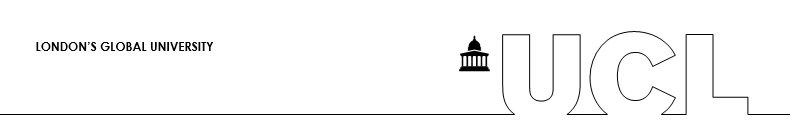
\includegraphics[width=1.2\textwidth]{images/Coversheet_Header.png}}
	
			\vspace{15mm}
			
			\begin{center}
				{\Huge \textbf{COMP0037 \\ \vspace{10mm} Report}}
			
				\vspace{8mm}
			
				\begin{spacing}{1.8}
					{\huge Path Planning in a Known World}
				\end{spacing}
		
			
				\vspace{12mm}
			
				{\LARGE \textbf{Group AS}}
				
				\vspace{10mm}
				
				\begin{tabular}{ll}
					\underline{\textbf{Student Name}}  & \hspace{4mm} \underline{\textbf{Student number}} \vspace{2mm} \\
					Arundathi Shaji Shanthini & \hspace{4mm} 16018351 \\ 
					Dmitry Leyko & \hspace{4mm}  16021440\\ 
					Tharmetharan Balendran & \hspace{4mm} 17011729\\ 
				\end{tabular}
				
				\vspace{13mm}
				
				\begin{tabular}{ll}
					\textbf{Department:} &  Department of Electronics and Electrical Engineering\\ \vspace{3mm}
					\textbf{Submission Date:} &  25\textsuperscript{th} of February 2020
				\end{tabular}
			\end{center}
	\end{titlepage}
	%%%%%%%%%%%%%%%%%%%%%%%%%%%%%%%%%%%%%%
	
	\pagebreak
	
	\tableofcontents
	
	\pagebreak
	
	%%%%%%%%%%% PART 1 %%%%%%%%%%%%%%%%%
	\section{Implement and Investigate Properties of Path Planning Algorithms}
		
		\subsection{Path Planning Algorithms}
				
			\begin{figure}[H]
				\renewcommand\thefigure{1.1}
				\centering
				
				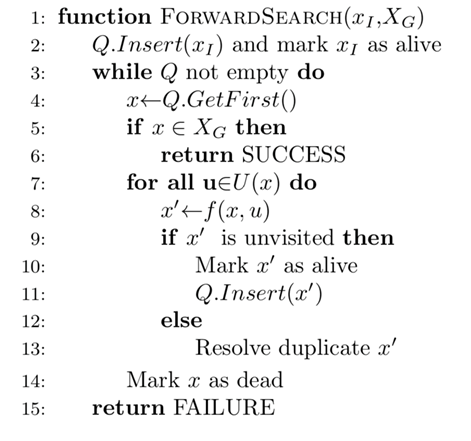
\includegraphics[scale=0.6]{images/general_forward_search_pseudocode.png}
				\caption{The general forward search algorithm pseudo-code. }
			\end{figure}
			
			All of the path planning algorithms have the same backbone and can be summed up into 15 lines of pseudo-code shown in Fig 1.1. This algorithm describes the process of finding a path from a cell ($x_I$) to a goal cell ($X_G$). This general algorithm is called the general forward search algorithm and is implemented in the \textbf{GeneralForwardSearchAlgorithm} class. All planners that are implemented inherit from this class through the \textbf{CellBasedForwardSearch} class. The search algorithm is similar for all the planners and has also been implemented in the same \textbf{GeneralForwardSearchAlgorithm} class. What differs between the planners is the type of queue that is used and the implementation of the \textbf{resolveDuplicate} function. These properties and functions are defined in the classes of each of the individual planners. It should also be noted that a class named \textbf{PlannerBase} is also present. This function consists of abstract functions and variable decelerations as well as functions required for visualisation of the planned path. The high-level working of the planners we implemented and their properties are described below.
			
			\subsubsection{FIFO - Breadth First Search}
	
				This algorithm works by selecting a particular cell and exploring its neighbours first. It would then pivot around those neighbours to explore each of their neighbours. Layer by layer it will explore all the cells on the graph network until it reaches the goal. The next cells to be considered are chosen by first considering the cell directly underneath and then considering the neighbouring cells going anti-clockwise. This way of allocating the next set of cells to be considered, is the same for all algorithms. The Breadth First Algorithm uses a queue to keep track of the order of the exploration in the network. If a particular cell shows itself twice to the algorithm, it will use the first instance of it ignoring the second. The first path that reaches the finishing cell is the final output path, no mater of the cost. The name First in First Out (FIFO) comes from the type of queue implemented in this search algorithm. The next cell to be considered at any point is the one that was added the first out of all the cells in the queue.
				\\
				The Breadth First Search Algorithm utilizes a normal unsorted queue and was implemented using the python \textbf{deque} class. For the pushing and popping of cells, the in-built \textbf{append} and \textbf{popleft} functions were utilized. In the case a cell that was already visited is re-visited in the Breadth First Search, nothing is considered. Therefore the \textbf{resolveDuplicate} function is an empty function in this case. 
				\\
				The biggest advantage of FIFO is that it will never get stuck in a blind alley. If there is a solution it will find it. If there are multiple solutions, it will find one with the least steps. The memory usage can be large as it stores all the cells that it visits. If the solution is far, it might take a lot of time to find, as well as that the FIFO algorithm does not guarantee optimality. In the worst case scenario with the FIFO algorithm will consider every possible cell and edge. Therefore the complexity can be expressed as $O(V+E)$ where V is the total number of vertices/cells and E is the total number of edges in the graph. 
			
			\subsubsection{LIFO - Depth First Search}
			
				This algorithm is very similar to the Breadth First Search. Starting from the initial cell, the algorithm adds cells to the queue in the same fashion as previously described. Where Depth First differs is in the fact that instead of using a first in first out queue, a last in first out (LIFO) queue is utilized. As a result at any given moment the next cell to be considered is the last one that was added to the queue. 
				\\
				The depth first algorithm utilizes a normal python \textbf{list} class alongside the \textbf{pop} and \textbf{append} functions. Once again, in the event a cell is revisited the first instance is considered. This results in an empty implementation of \textbf{resolveDuplicate}. 
				\\
				Once again, the depth first algorithm does not grantee the optimal path. In fact, due to the nature of the LIFO queue, the computed paths tend to be chaotic with many zig-zag features. Similarly to the Breadth First Algorithm, in the worst case scenario the Depth first algorithm will consider each cell of the graph. This means that once again the complexity of the algorithm can be expressed as $O(V+E)$ where V is the total number of vertices/cells and E is the total number of edges in the graph.
			
			\subsubsection{Greedy Search}
			
				The Greedy Search Algorithm starts at the first cell and adds neighbouring cells to the queue. The type of queue used in this algorithm is a priority queue with the priority value being the euclidean distance between the cell and the goal. This means that the cells in the queue are sorted by their euclidean distance to the goal. As a result when a cell is popped from the queue it will be the cell with the lowest euclidean distance to the goal (out of the cells in the queue). As a result the algorithm will consider the cells closer to the goal first. This can drastically reduce the number of cells that are considered resulting in lower computational requirement.
				\\
				The greedy algorithm was implemented using a priority queue from the \textbf{PriorityQueue} library. Along with the built-in \textbf{put}, \textbf{get} and \textbf{empty} functions it was relatively easy to implement the priority queue and thereby the greedy algorithm. Once again in the case a cell is revisited nothing is done, meaning that the \textbf{resolveDuplicate} function is empty.
				\\
				The biggest advantage of the greedy algorithm is its easy implementation and its efficiency in simple cases. In maps with minimal/no obstructions, the greedy algorithm is able to find a path with significantly fewer cells visited compared to breadth first and depth first planners. However the optimality of the path is not guaranteed.
				
			\subsubsection{Dijkstra's}
			
				This algorithm works by first setting the values for distances to every cell to infinity. Once the starting cell is specified, its cost to go value is set to zero and it is set to have no parent cell. The algorithm then explores the neighbours of the starting cell and records the distance to each. Once this is done, the neighbouring cells are added to the queue which is once again a priority queue with the priority value being the cost to go to the cell. The next cell to be considered is the cell with the lowest cost to go (from the cells in the priority queue). The algorithm will continue until the queue is empty. The cost to go is calculated using the L-stage additive cost which considers the terrain cost as well as edge costs that are present. 
				\\
				Once again the same priority queue as implemented in the greedy algorithm was utilized with changes to the priority value. In addition to that, the class \textbf{DijkstraPlanner} inherits from another class \textbf{DynamicPLanner}. This is due to the fact that Dijkstra and A* planners are both dynamic planners and not only use the same queue but only differ by the addition of heuristics. Therefore, the priority queue and functions associated with it are common to both and can therefore be shared. Additionally, the \textbf{resolveDuplicate} function is also shared amongst the two planners. In the case a cell is revisited, the existing cost to go and the new proposed cost to go are compared. If the new cost to go is smaller, then the cell's parent and cost to go are updated to reflect this. 
				\\
				The main advantage of utilizing Dijkstra's is the fact that the optimality of the path is guaranteed. In addition to this, Dijkstra computes the path to the goal from not only the start cell but all cells that have been visited. This means that if at a later date another path to the same goal is required, the algorithm doesn't have to restart from beginning. The main disadvantage is that the algorithm is computationally intense having a time complexity of $O(E\log(V)+E)$ where V are vertices/cells and E are edges. 
				
			\subsubsection{A* Search}
			
				This algorithm works in a similar way to Dijkstra’s however it additionally uses a heuristic to influence the way it selects which cells to explore and visit. Heuristics used in our assignments are: a non-negative constant value, the euclidean distance to the goal, the octile distance to the goal and the Manhattan distance to the goal. The algorithm is similar to Dijkstra and as previously discussed the two planners inherit from the same \textbf{DynamicPlanner} class. When adding a cell to the priority queue, the heuristic value is computed for that cell and it is summed to the L-stage additive cost. This means that the heuristic influences the position of the cell in the priority queue and therefore may change the order in which cells are considered. The heuristics bias the considered cells such that cells closer to the goal are considered first meaning that fewer cells my be visited in the process of finding the final path.
				\\
				The euclidean distance is the straight line distance between two points expressed as shown in Eq. X. 
				
				\begin{equation}
					\hat{G}_{k} = \sqrt{(x_k-x_G)^2+(y_k-y_G)^2}
				\end{equation}
				
				Depending on robot movement restrictions, the heuristic may be altered to take this into account. For example, the octile distance is the minimal distance using horizontal, vertical and 45 degree diagonal trajectories. This corresponds to a robot that can move in 8 directions (N, NE, E, SE, S, etc...). The expression for computing this distance is shown in Eq. X.
				
				\begin{equation}
				\hat{G}_{k} = max(|x_k-x_G|,|y_k-y_G|) + (\sqrt{2}-1)min(|x_k-x_G|,|y_k-y_G|)
				\end{equation}
				
				Similarly to the octile distance, the Manhattan distance computes the shortest distance between two points using only vertical and horizontal trajectories. This corresponds to a robot that can move in 4 directions (N, E, S, W). The expression to compute this distance is shown in Eq. X. 
				
				\begin{equation}
				\hat{G}_{k} = |x_k-x_G|+|y_k-y_G|
				\end{equation}
				
				Given that the chosen heuristic is non-zero and never overestimates the cost to the goal, the heuristic is said to be admissible. In the case that a heuristic is admissible, it also follows that the computed path will be the optimal path. The most optimal heuristic will be the one that doesn't just approximate the distance to the goal but rather is exactly equal to the cost to the goal. In this case, the number of cells visited will be minimal and the optimal path will also be identified. However, this is non feasible as computing the actual cost to goal is computationally intense. In the case a heuristic is inadmissible, the optimality of the path is not guaranteed.
				\\
				In addition to the type of heuristic used, the A* planner can be further customized and tuned by using a weighting parameter on the heuristic. This weighting parameter influences the number of cells searched by the planner and the optimality of the found path. By choosing a weighting factor greater than 1, the algorithm prioritizes cells closer to the goal. However this also means that the weighted heuristic may become inadmissible and therefore not necessarily derive the optimal path. On the other hand, a weighting factor lower than 1 explores more cells than the un-weighted heuristic but will return the same optimal path. This additional exploration of cells may only be useful, if paths from those cells to the goal are required at a later time. 
				\\
				As previously discussed, the implementation of the A* algorithm is very similar to the implementation of Dijkstra. The main difference is the addition of the \textbf{calc\_heuristics} function that computes the heuristics. The choice of heuristic is defined in the launch file and can be determined as a argument when launching the node using roslaunch.
				\\
				The time complexity of the A* algorithm can be expressed as $O(E)$ where E is the total number of edges in the graph.
				
		\subsection{Algorithm Performance}
			\subsubsection{Metrics to Quantify Performance}
				To measure and evaluate the performance of the planners, five metrics were utilized: Path cost of optimal path, total angle turned, maximum queue cardinality, total number of cells visited and path cardinality. The path cost refers to the total cost of traversing the path returned by the planning algorithm. The total angle turned corresponds to the sum of the absolute value of all of the individual turns the robot has to make. The maximum queue cardinality is the maximum number of elements the queue had at any point in the planning process. This reflects the memory usage of the algorithm. The total number of cells visited is as the name implies and reflects the time taken for the planner to compute the path. Finally the path cardinality is a count of the number of individual waypoints in the path.
				\\
				To compute the cost of the path the L-stage additive cost between the parent of a cell and the cell is computed for every cell on the path. This will give the total cost of traversing the path. This is done in the \textbf{extractPathEndingAtCell} function which starts from the goal and backtracks to the initial cell, cell by cell to compute the planned path.
				\\
				To compute the total angle turned, the trajectory of the robot was considered. By trajectory what is meant is the direction the robot is facing/moving at any point in the path. This is computed by taking the arctangent of the ratio between the difference in y coordinates and the difference in x coordinates of the cells. Whenever there is a change in trajectory, the difference in the trajectory will give the turned angle. The sum of the absolute values of these angles corresponds to the total angle turned. 
				\\
				The maximum queue cardinality was easily implemented by checking the size of the queue every time a new cell was added and updating the maximum value if it is exceeded.
				\\
				The total number of cells visited is computed easily in the implementation of the general search algorithm. Every time a new cell is added to the queue, the number of cells visited is incremented by one. 
				\\
				The path cardinality is computed by taking the length of the planned path which corresponds to the number of cells on the planned path. This is done after having traversed through all cells from the goal to the initial cell. 
				\\
				These metrics should give a good measure of how well a planning algorithm performs. A lower path cost represents a more optimal path while a larger number of cells visited may imply a inefficient algorithm. 
			\subsubsection{Evaluating Performance of Algorithms}
			
				\begin{figure}[H]
					\renewcommand\thefigure{1.2}
					\centering
					
					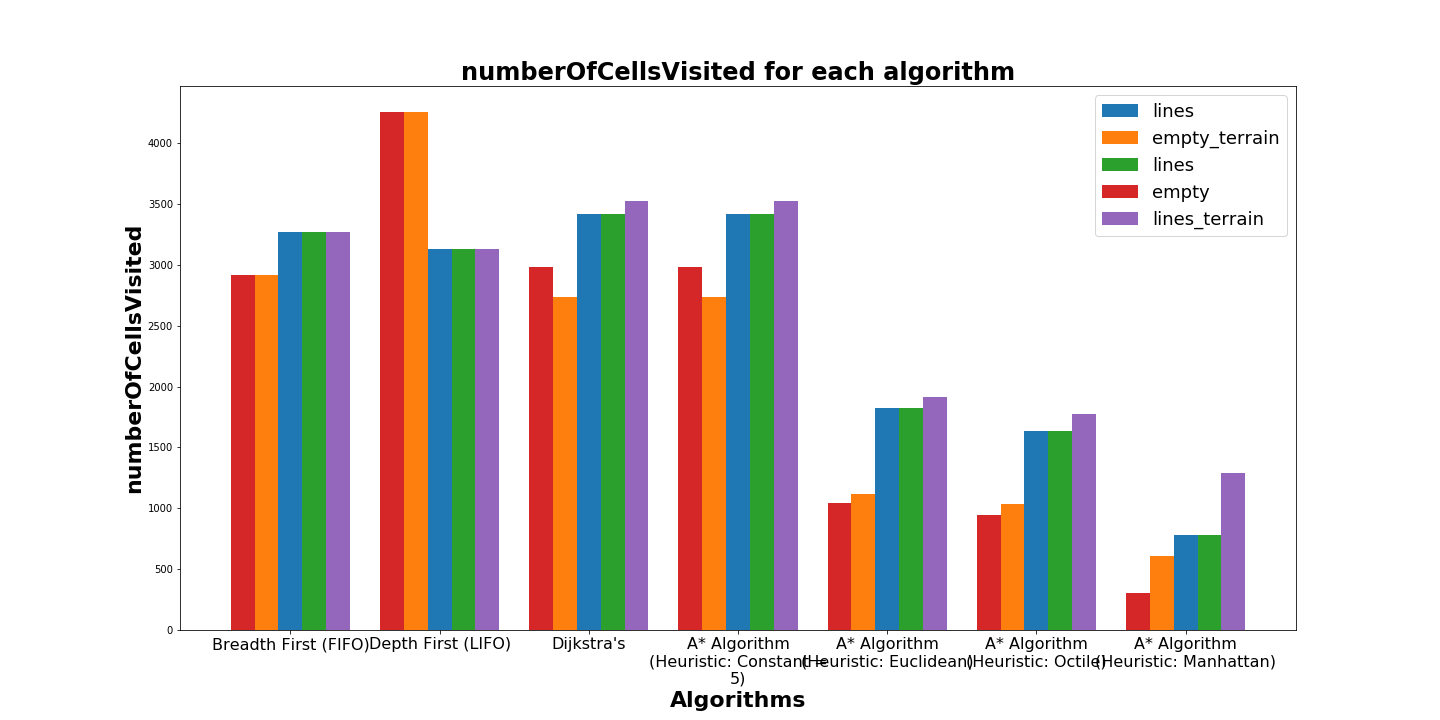
\includegraphics[scale=0.3]{"images/numberOfCellsVisited for each algorithm.png"}
					\caption{The Number of Cells visited by each of the algorithm during path planning on a variety of maps.}
				\end{figure}
			
				\begin{figure}[H]
					\renewcommand\thefigure{1.3}
					\centering
					
					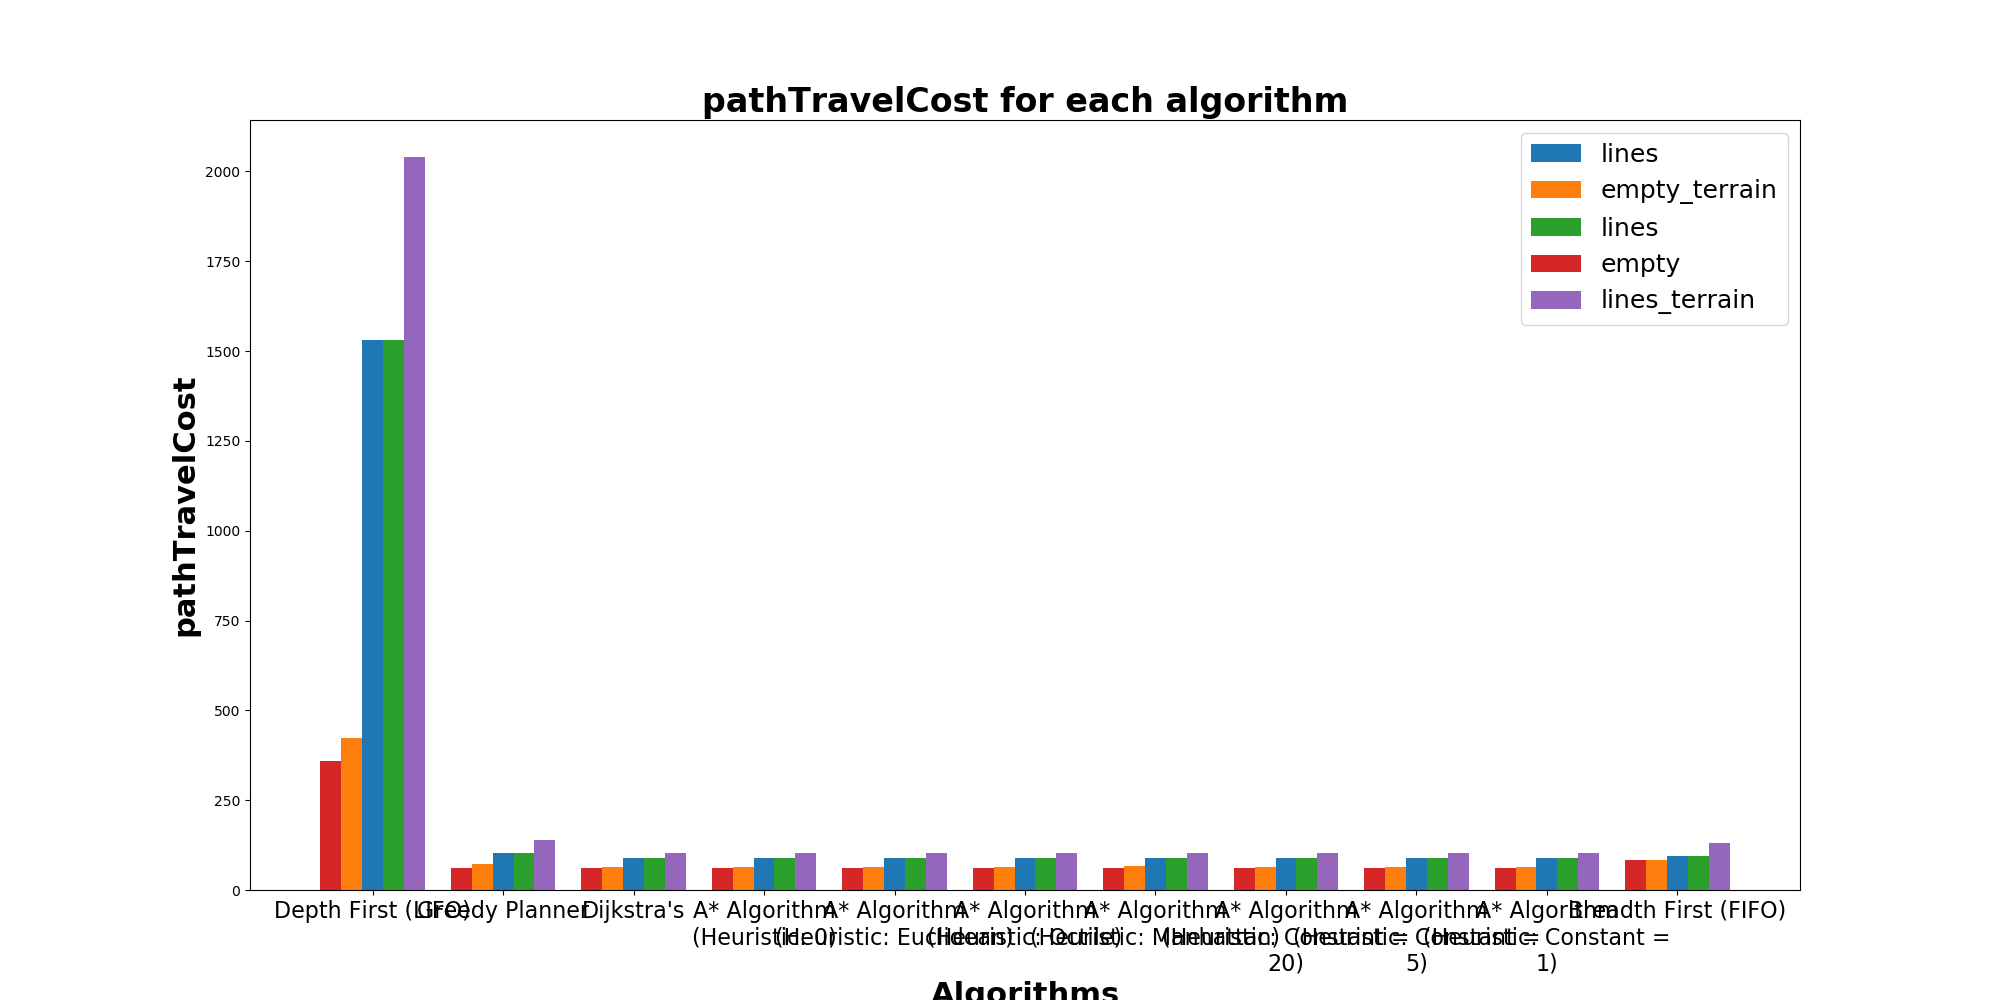
\includegraphics[scale=0.3]{"images/pathTravelCost for each algorithm.png"}
					\caption{The cost of traversing the path that was found by the planning algorithm.}
				\end{figure}
			
				\textbf{FIFO - Breadth First Search}
				\\
				The Breadth First Algortihm performed poorly. The path cost of the derived path mostly wasn't optimal and especially on maps with a terrain cost superimposed, the algorithm performed poorly. In addition to this, the planner visits a large number of cells in comparison to the path cardinality implying a inefficient search algorithm. How-ever the maximum cardinality of the queue was relatively small suggesting a relatively small memory usage. Due to the simple nature of the planner, the complexity of the path was low resulting in minimal turns.
				\\
				\textbf{LIFO - Depth First Search}
				\\
				This algorithm was by far the worst performing algorithm. This algorithm consistently returned the path that had the highest path cost out of all the planning algorithms. Additionally, it also had exceptionally large number of turns and bends. However, the number of cells traversed was comparable to the other algorithms and relatively low for the given path cardinality. Compared to the performance of the other planners, the depth first planner is completely inefficient and returns a chaotic path.
				\\
				\textbf{Greedy Algorithm}
				\\
				The greedy algorithm performed extremely well in most cases. It consistently had the lowest number of cells visited while searching for the path. However it had a slightly higher path cost which is most prominent in the lines\_terrain map. This is to be expected as the greedy algorithm (similar to breadth and depth first) do not have a notion of path cost while they are searching for the path. This is most prominent when the terrain cost isn't uniform. The maximum queue cardinality was neither exceptionally high nor exceptionally low when compared to that of the other planners that were implemented. 
				\\
				\textbf{Dijkstra's Algorithm}
				\\
				Dijkstra's Algorithm produced the path with the minimal path cost as expected. This means that it finds the optimal path. Besides this, the algorithm visited a relatively large number of cells while searching for the path meaning that the search algorithm is slightly inefficient. 
				\\
				\textbf{A* Algorithm}
				\\ 
				The A* Algorithm was implemented with the 4 heuristics that were previously discussed. When the A* algorithm has a heuristic of zero, the planner is identical to Dijkstra's Algorithm. With the addition of a constant heuristics (i.e. a non-negative constant), the A* algorithm is still identical to Dijkstra's. This is due to the fact that there is no favouring in which cell should be considered first as all cells are assigned the same heuristic values. Even though these scenarios were simulated and observed for all of the given maps, these variations of A* are not illustrated in the graphs in Fig. X.X to avoid repetition. It was confirmed that these cases were exactly identical to A* and one variation of a constant with value of 5 is shown for comparison.
				\\
				The euclidean distance heuristic acted as intended. Due to its admissible nature, the addition of the heuristic did not alter the path cost in any of the cases. However it did alter the number of cells visited; In all of the cases, the A* algorithm with euclidean distance heuristic performed better (having visited less cells) than Dijkstra's Algorithm. This is to be expected as the whole purpose of heuristics is to limit the number of cells visited by biasing cells to be higher up in the priority queue. However, as the robot in our case is able to move in 8 directions (octile movement), the euclidean heuristics significantly under-estimates the distance to the goal. Therefore the heuristic is not optimal.
				\\
				The octile distance heuristic corresponds to a robot moving in 8 directions just as the one in the simulations. This heuristic will more closely approximate the true cost to the goal cell compared to the euclidean heuristic; the value of the distance will be higher but still less than (or equal to) the actual distance. As this approximation of the distance is larger, the number of cells visited will be fewer. This is due to a higher value of the heuristic meaning a larger bias towards the cells that are closer to the goals which in turn results in these cells being visited first. As the heuristic is still admissible, the path that is obtained is the optimal path and as a result of the octile heuristic it also achieves this having visited as many cells. 
				\\
				The last heuristic that was implemented was the Manhattan heuristic. This heuristic is an even larger approximation of the distance to the goal resulting in a further reduction in the number of cells visited. However as this heuristic is not admissible in the case of an octile robot, it cannot guarantee that the returned path will be the optimal path. Throughout the maps that were given to us, the Manhattan algorithm performed well with a path cost close to if not identical to that of the optimal path. 
				
			\subsubsection{Planner Performance Prognosis}
			
				Out of the 4 heuristics available, the constant provides the same performance as Dijkstra’s, thus it gives an optimal solution in all the cases however it must explore many cells for it to happen, making the algorithm slow running. The Euclidean distance will also give an optimal solution in all possible maps. However it will explore the most cells out of the remaining heuristics. The octile distance will give the as good of performance in terms the path being optimal as Euclidean. It will have a better performance in terms of the number of cells explored. All of the aforementioned heuristics are admissible. Manhattan distance heuristic provides the best performance in terms of number of nodes explored, however it is an inadmissible heuristic thus there is a possibility of it giving a non optimal path which can be seen by closely studying the graphs in Fig. X.X.
				\\
				There is a possibility of creating a combination of these heuristics by averaging them out. The goal would be to reduce the number of nodes explored by the A* algorithm. For this it is possible to average out the heuristic values for Octile and Manhattan distances, giving a value in between. This could potentially create a better heuristic than octile in terms of cells explored, however there is no way of telling if it will be an admissible heuristic. Thus the octile distance would be the best heuristic to use as it will guarantee an optimal solution given a weighting of 1. 

	%%%%%%%%%%%%%%%%%%%%%%%%%%%%%%%%%%%%%%
	%%%%%%%%%%% PART 2 %%%%%%%%%%%%%%%%%
	\section{Implementation in ROS}
	
		\subsection{Implentation of Planning Algorithms}
			
			To investigate how these planning algorithm may be utilized and applied, the STDR simulator package in ROS was used. This is a 2D simulation platform in which maps and terrains may be loaded and simulated. Using the factory map that was provided along with a list of goals, we were able to simulate the movement of the robot. To investigate how well the robot was traversing the path, we implemented the following metrics: time taken to traverse the path, total distance travelled and total angle turned. 
			
		\subsection{Comparison of planners}
		
		\subsection{Description of Robot Controller}
		After implementing the algorithm and evaluating the different paths obtained from the different algorithms, on running the STDR simulation it was noticed that robot followed the path but it was rather very slow. It was realised that this was due to the deliberately inefficient controller provided and hence some efforts were put into attempting to improve the controller.
		The low-level controller provided to us implemented a proportional controller. On playing around with the values of the gain and observing the velocity values being published it was understood that there is a lot of room for improvement as the velocity values being published were much below even 1m/s. 
		
		As an improvement it was thought that implementing a PID (Proportion-Integral-Derivative) controller would be a better than the Proportional controller that was initially implemented. PD controllers are a popular choice for controlling motors and hence it was thought that this might provide a better control. It was found that PID could be implemented as a rosnode and is ros package already available to use. However, due to lack of time to understand the working of this and implementing it on to this project the PID controller was implemented from scratch in the class \textbf{ControllerBase} by the function \textbf{pid\_controller(self, error, controller\_gains, afterFirst, delta\_t=0.1)}.This implements PID as per the following equation:
		\begin{equation}
			u(t)=K_P \; e(t) + K_I \int_{0}^{t}e(t')dt'+K_D \frac{de(t)}{dt}
		\end{equation}
		where,
		\begin{itemize}
			\item $K_P$ = Proportional Gain
			\item $K_I$ = Integral Gain
			\item $K_D$ = Derivative Gain
		\end{itemize}
	The values of these gains are determined by tuning them. However, without knowing the model of the robot it was not possible to use a tool like MATLAB or Simulink to tune the gains. Therefore, we adopted the method of empirical gain tuning and we systematically increased the gains of P, D and I components of the controller in the respective order till satisfactory improvement was achieved. The step repsonse plots and the error tracking plots were used to compare and determine any improvement in performance. Appendix \ref{appendix:Controller-tuning}
	
		Moreover, it is known that sampling rate can be a factor that affects the performance of the controller. If the sampling rate is not high enough to keep up with the rapid change in error value it can affect stability of the system. Practically, this is a known hardware limitation. However, in the case of this simulation, on experimenting with different values it was noticed that anything above 20Hz would give inconsistent time periods. 
		
		Further, it was noticed that because the path was represented by equidistant discrete waypoints even on a straight path the motion of the robot was a bit jittery and was not as smooth as we would desire it to be. This was corrected by reducing the number of waypoints that are input as reference to the controller. The function \textbf{simplifyPath(self, path)} in class \textbf{ControllerBase} implements this by removing all the waypoints which makes the same angle with its neighbour as does it neighbour with the cell after it, from the list.
	
	%%%%%%%%%%%%%%%%%%%%%%%%%%%%%%%%%%%%%%
	
	\newpage
	
	\appendix
	\appendixpage
	\addappheadtotoc
	\section{Class Inheritance}
	\subsection{Planner Inheritance}
	\label{appendix:planner}
	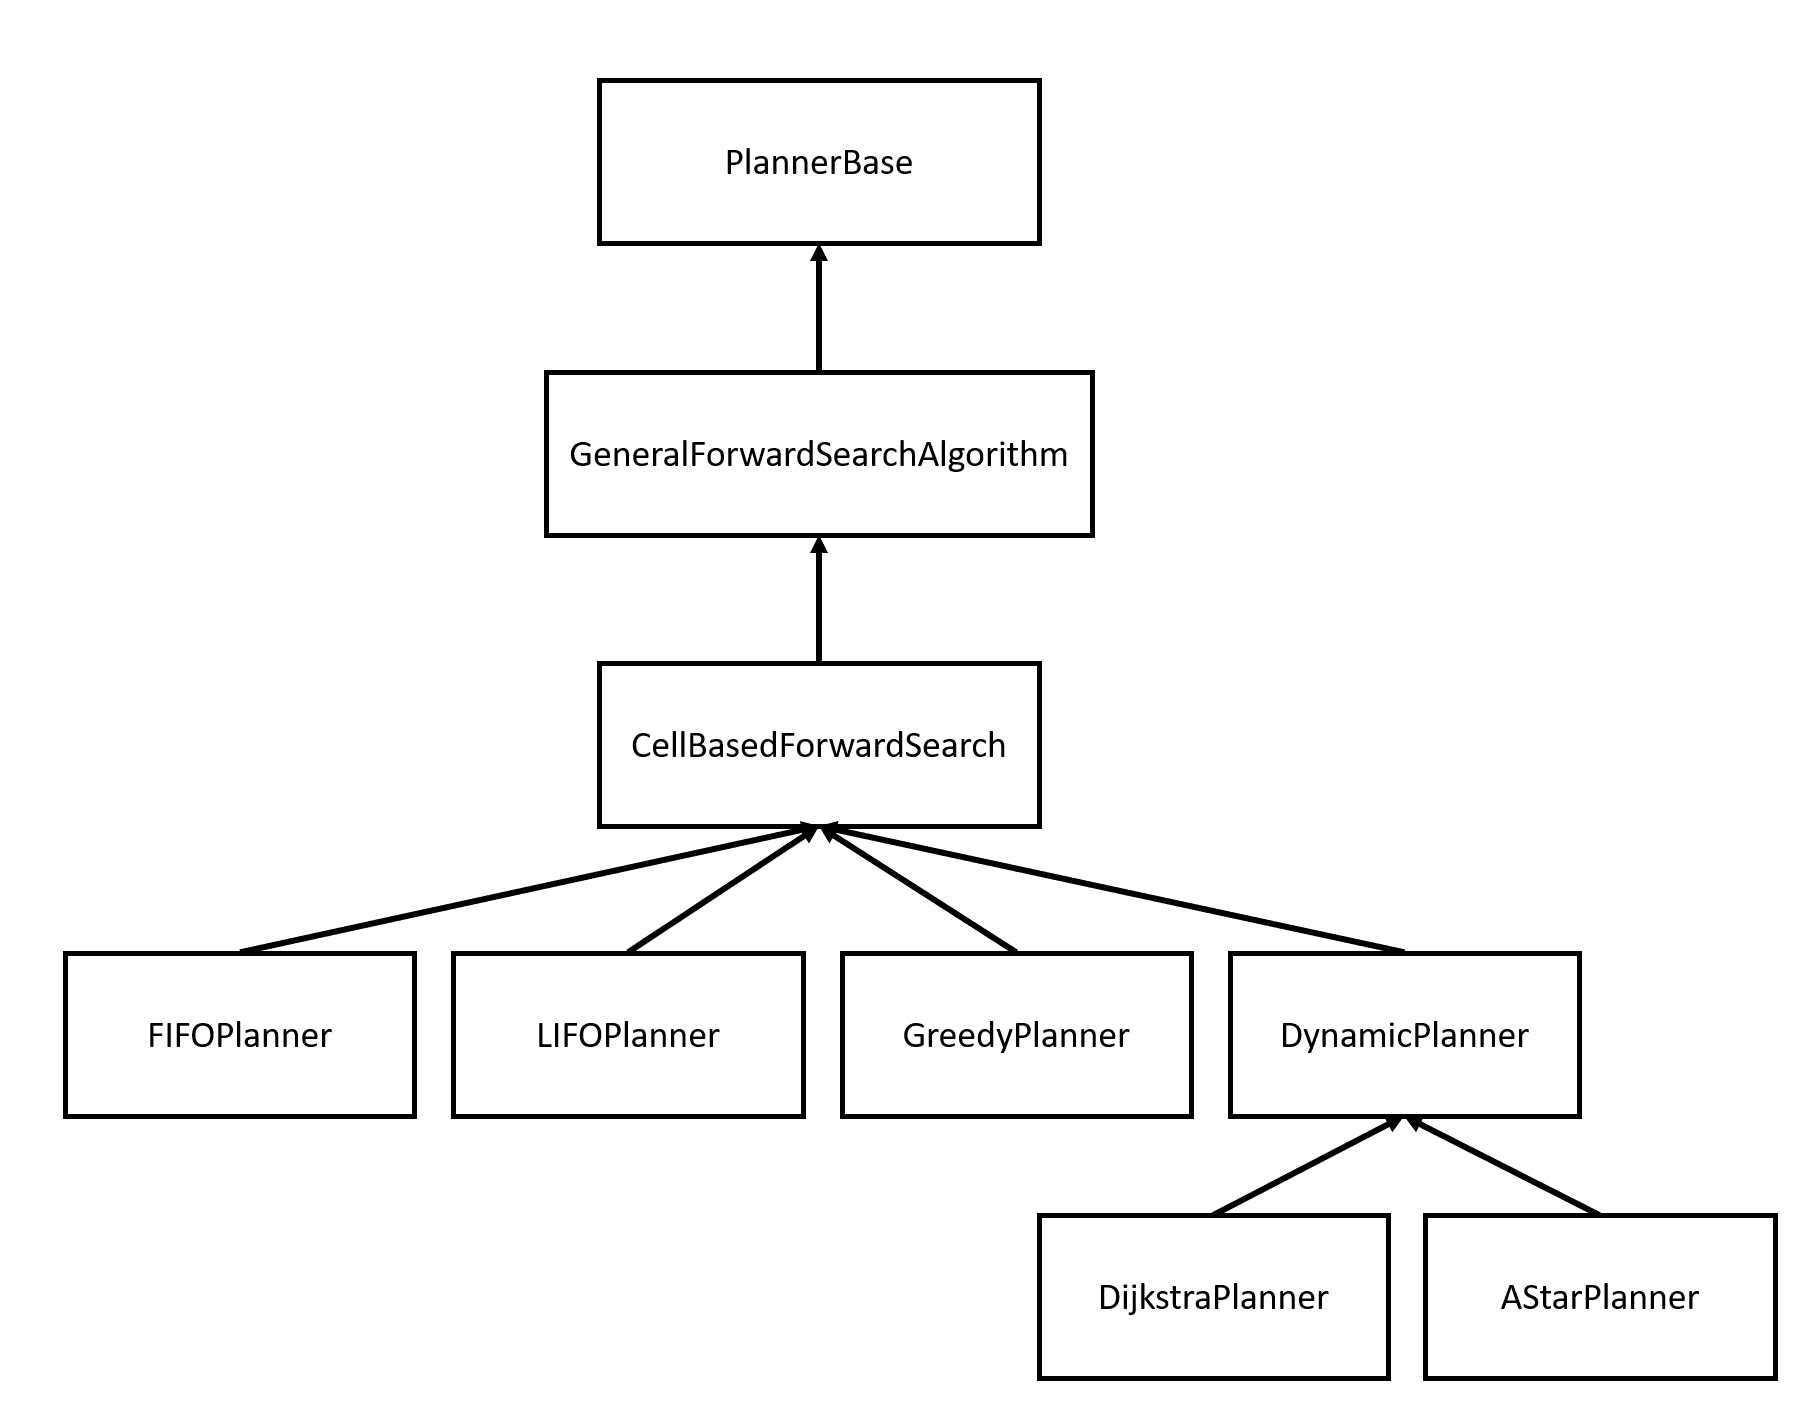
\includegraphics[scale=0.6]{images/planner_inheritance.png}
	\subsection{Controller Inheritance}
	\label{appendix:controller}
	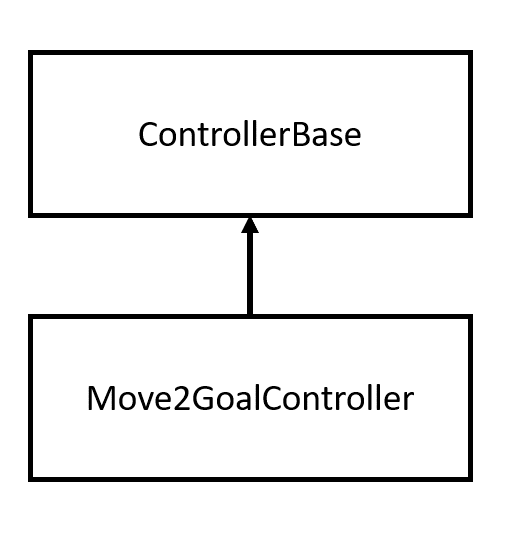
\includegraphics[scale=0.6]{images/controller_inheritance.png}
	\section{Tuning the Controller}
	\label{appendix:Controller-tuning}
	\subsection{Linear Distance Controller}
	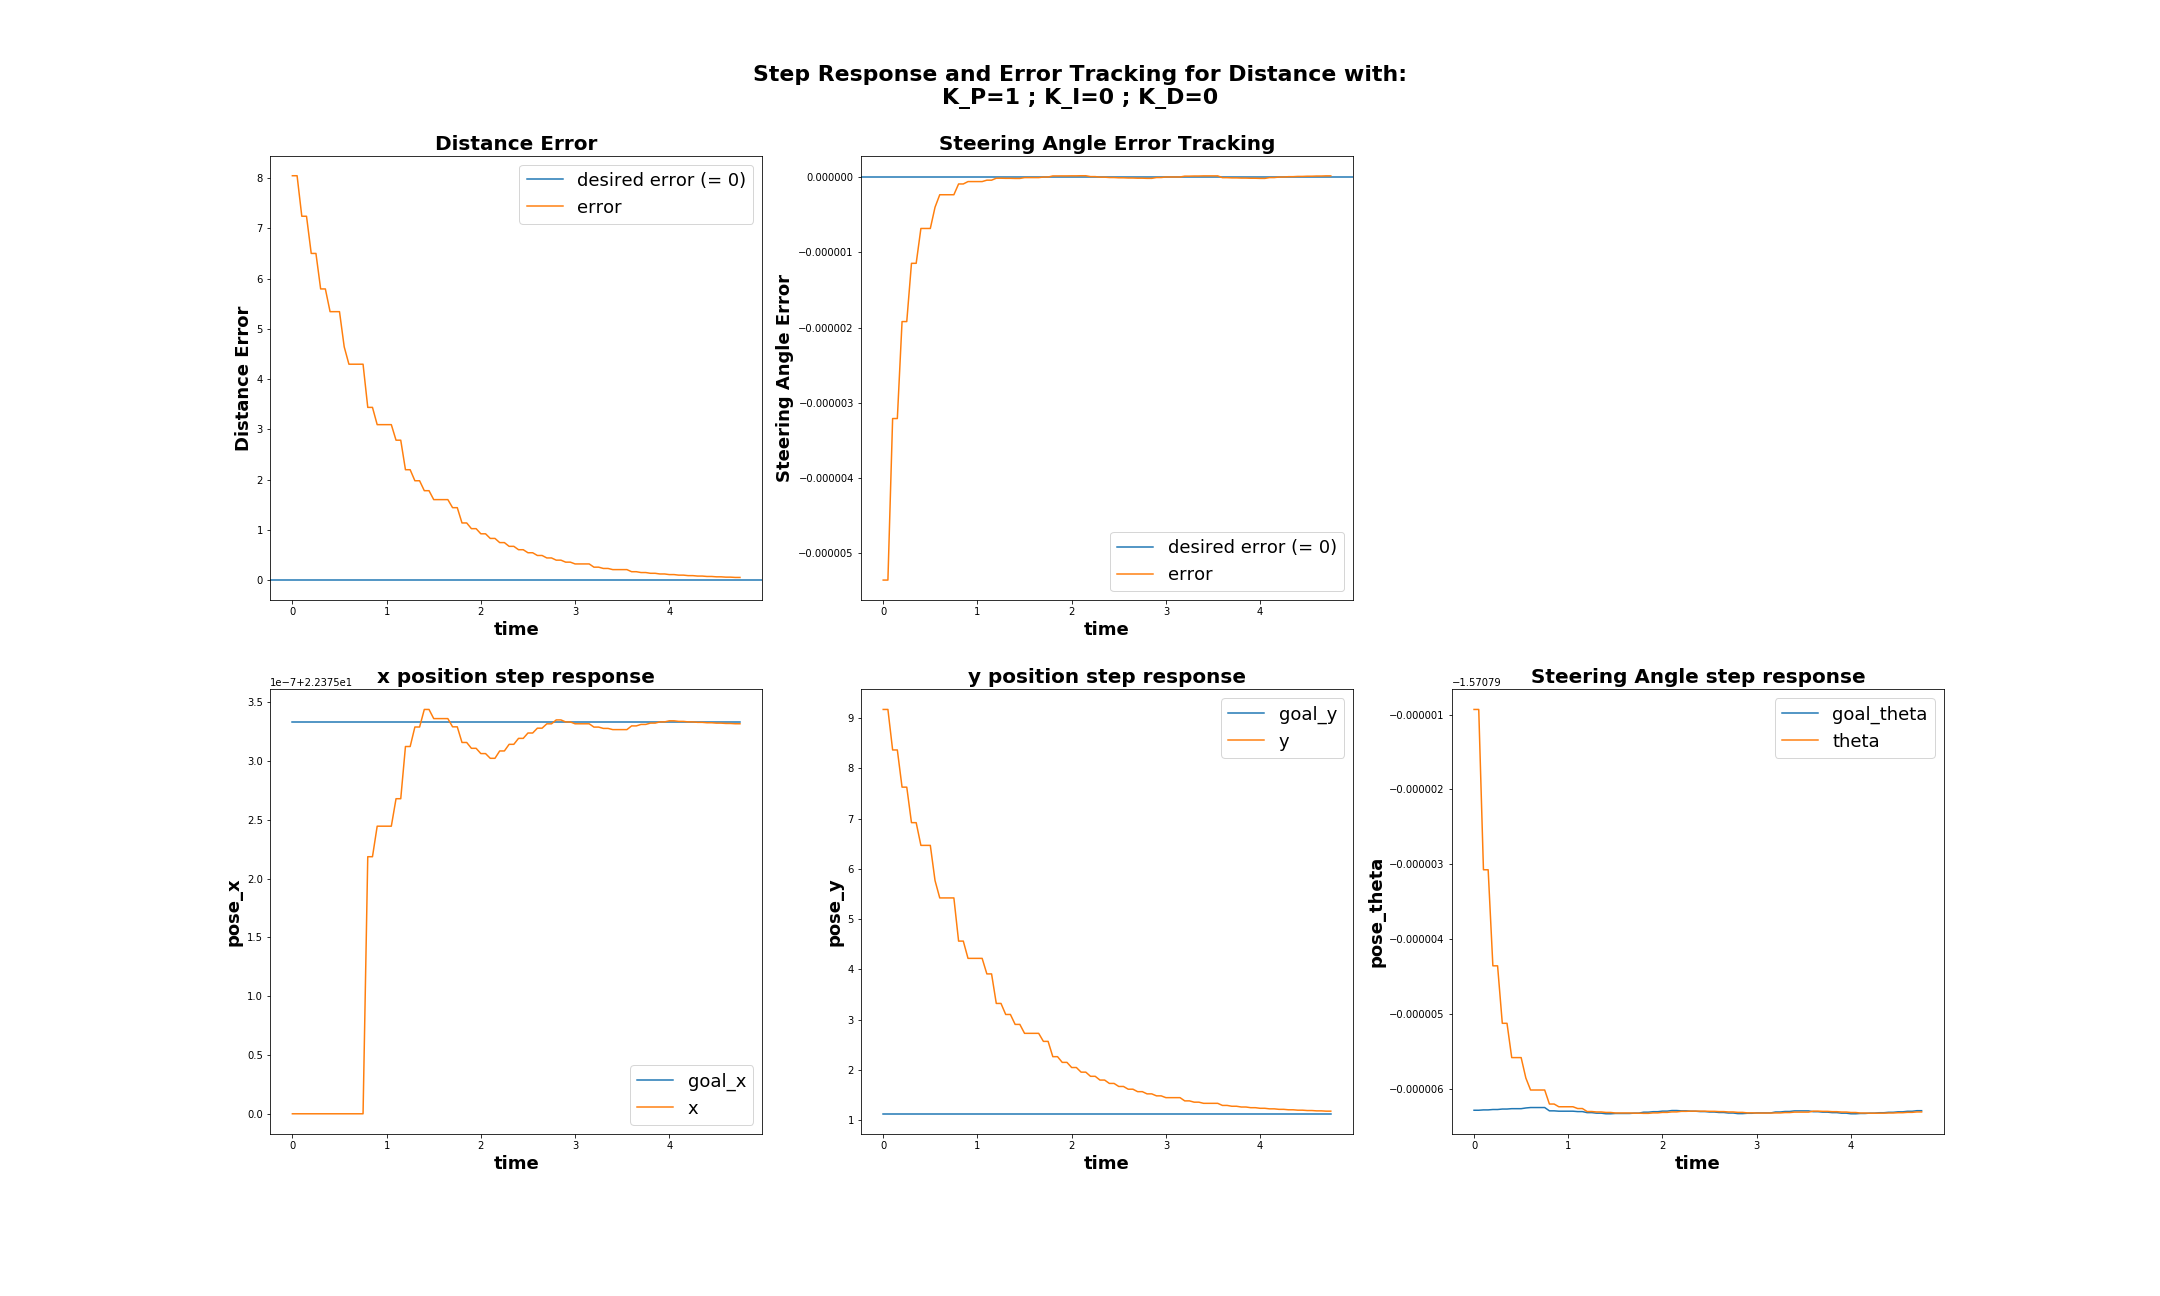
\includegraphics[scale=0.25]{images/control_dist_1_0_0.png}\\
	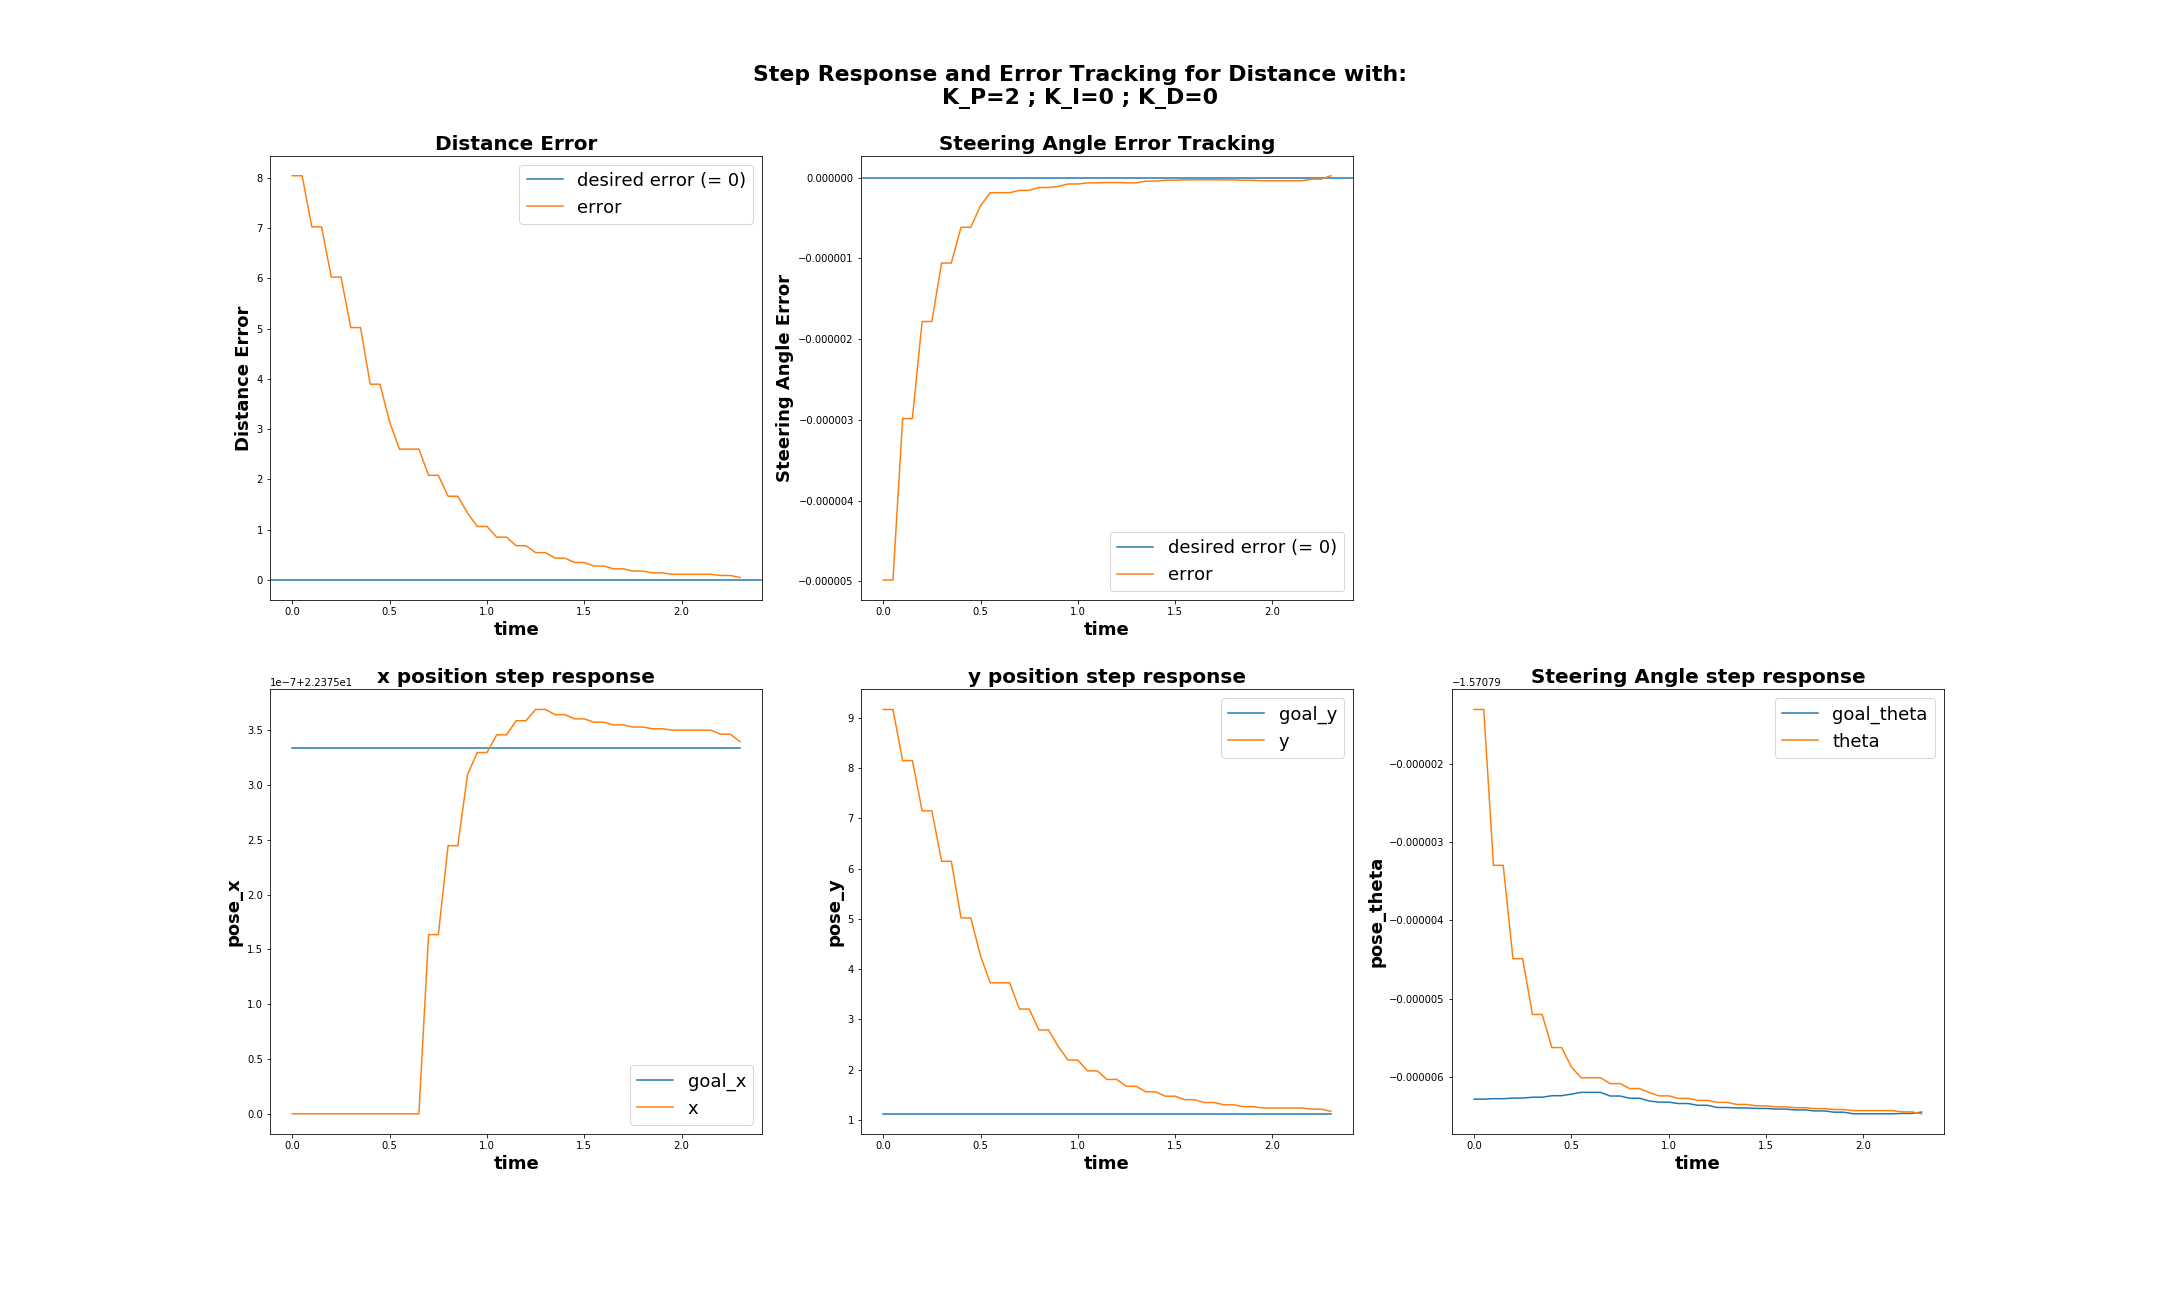
\includegraphics[scale=0.25]{images/control_dist_2_0_0.png}
	\\
	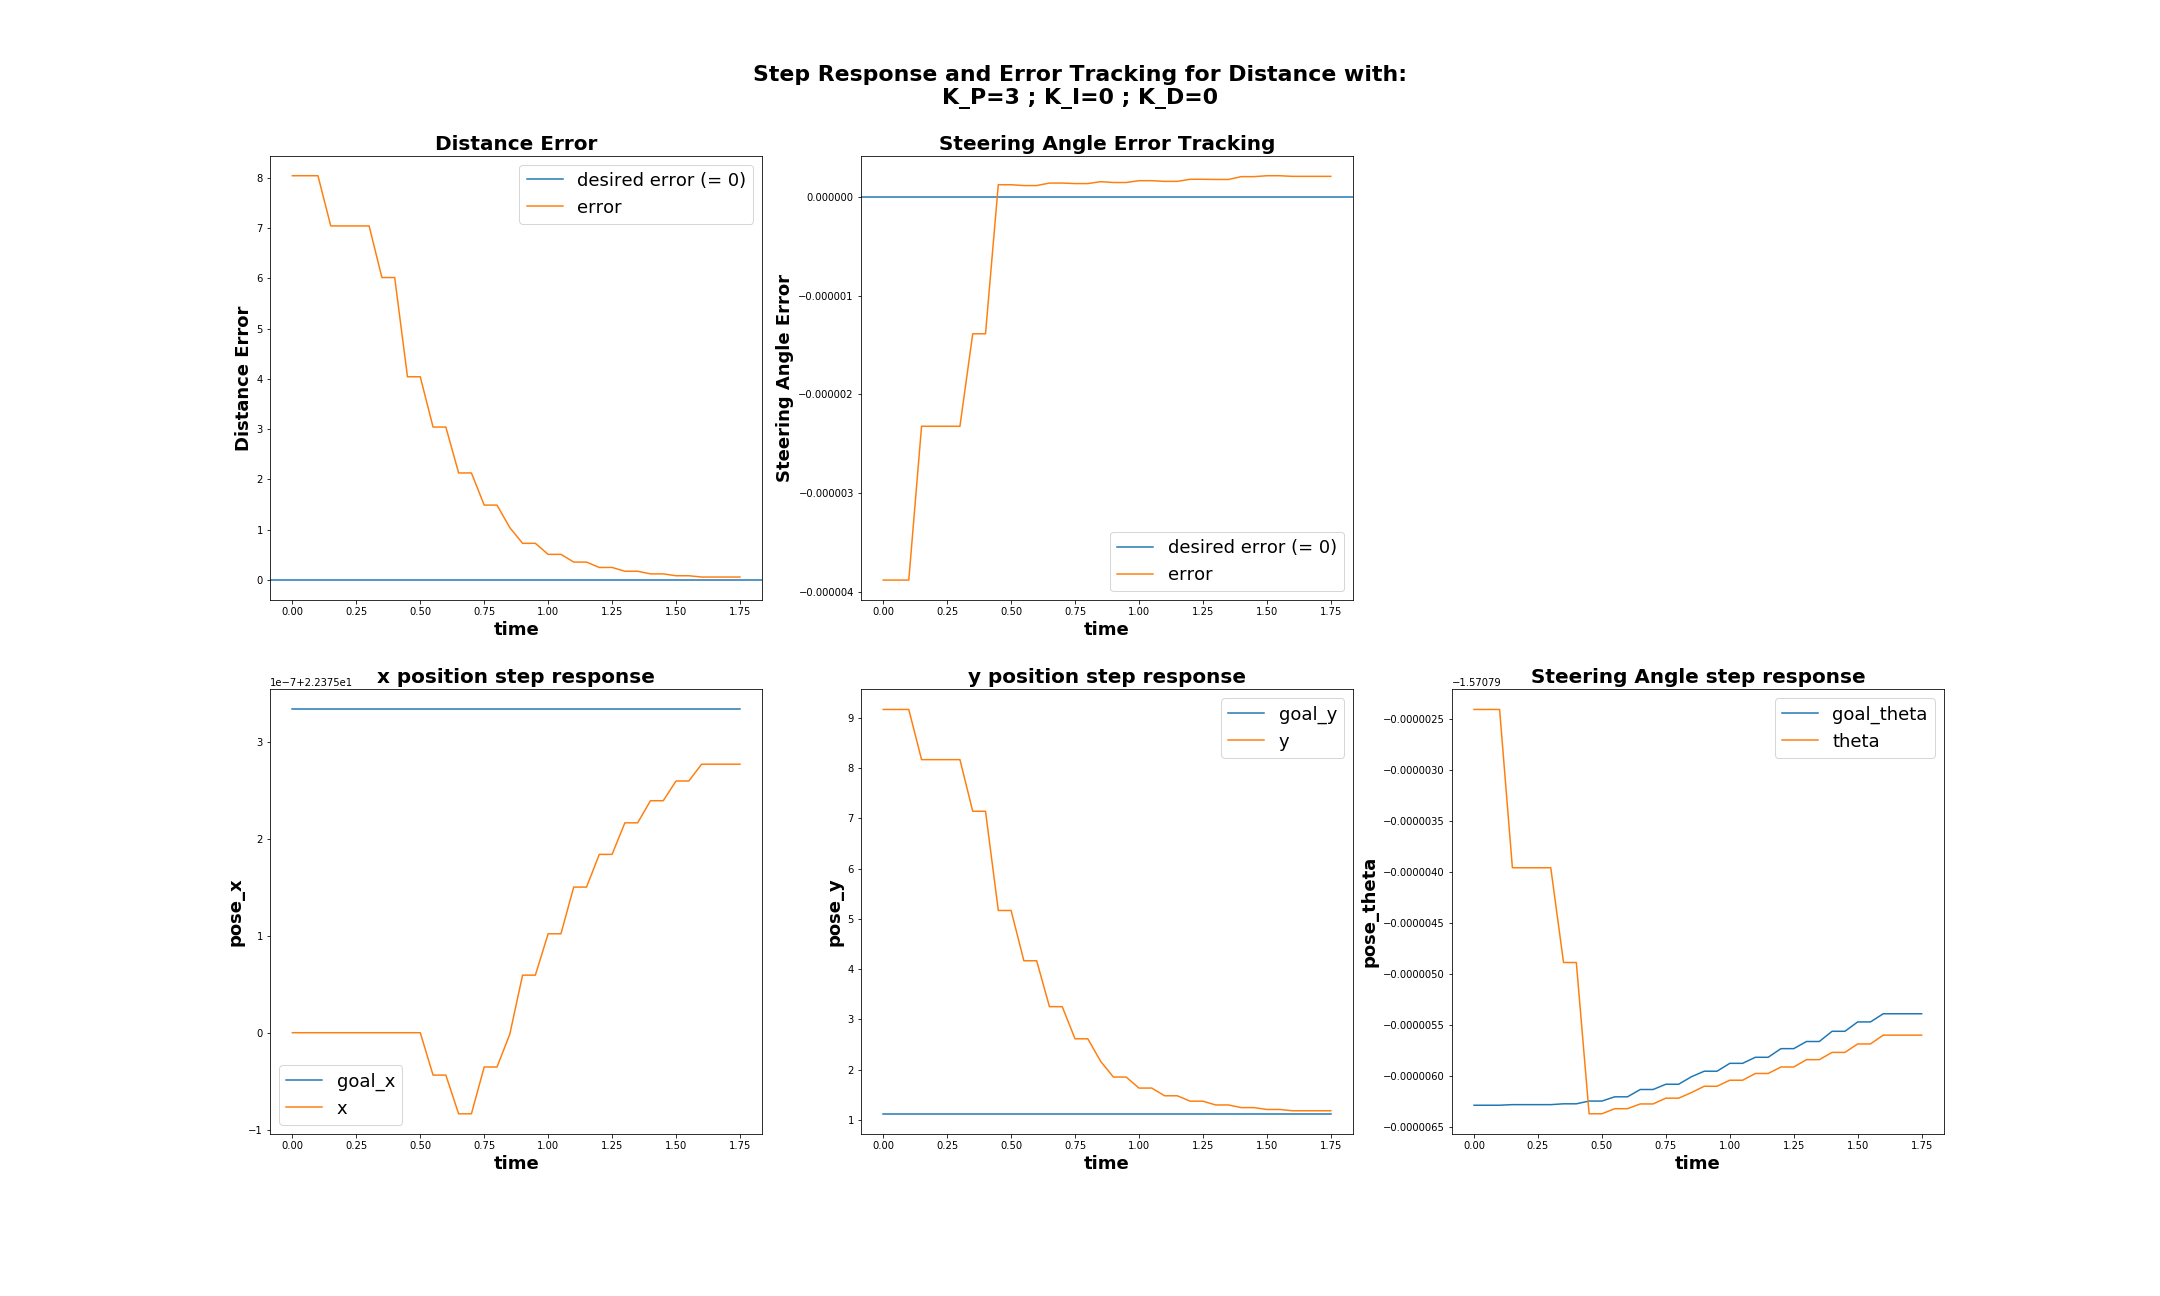
\includegraphics[scale=0.25]{images/control_dist_3_0_0.png}\\
	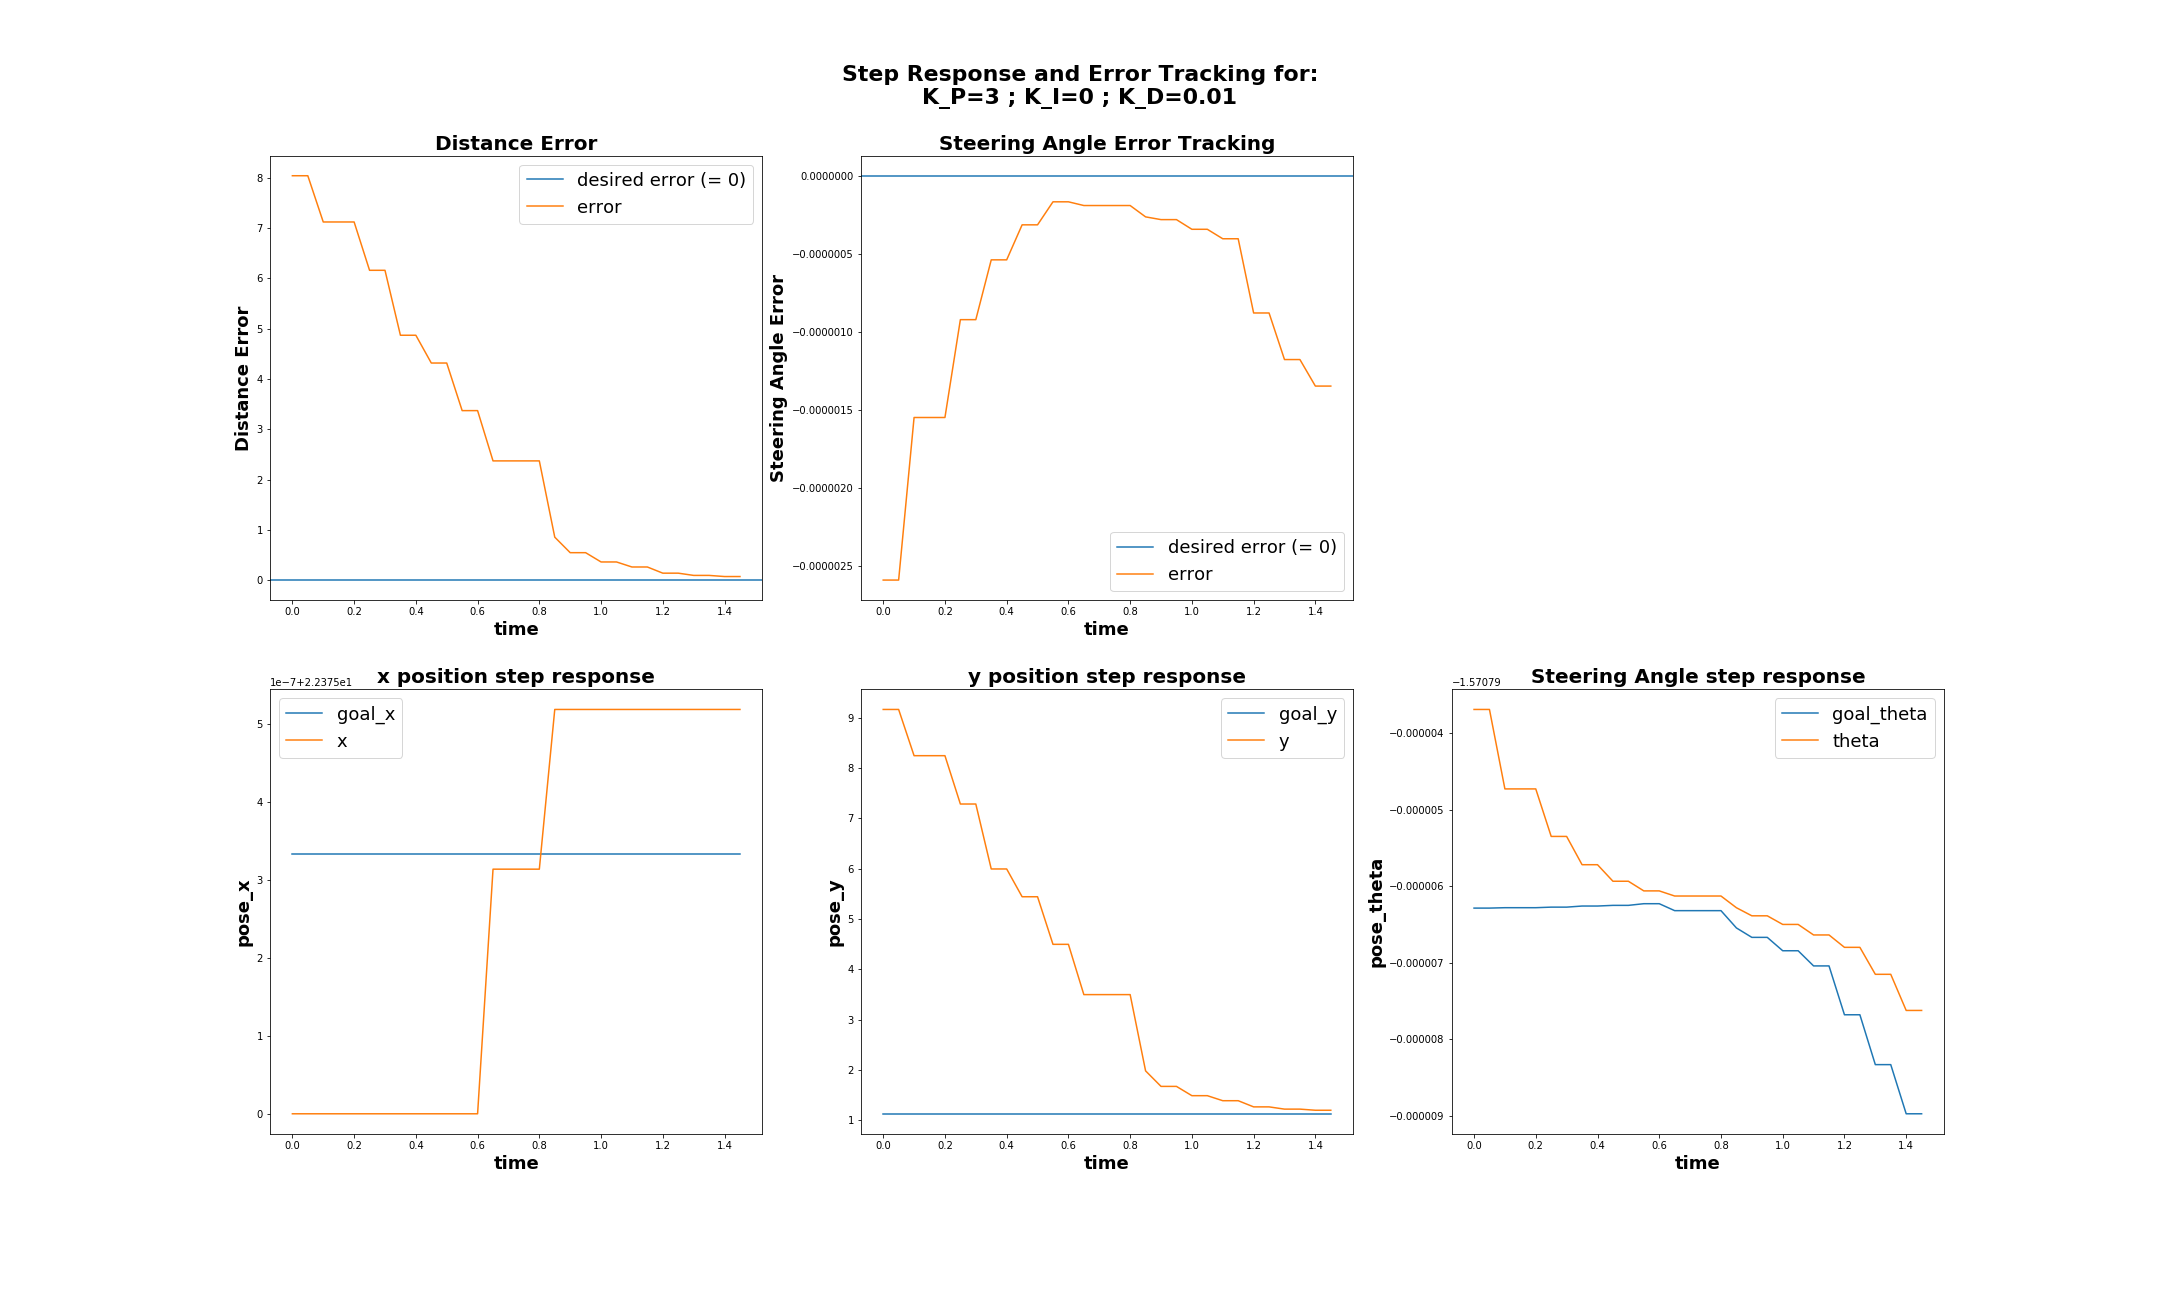
\includegraphics[scale=0.25]{images/control_dist_3_0_0.01.png}\\
	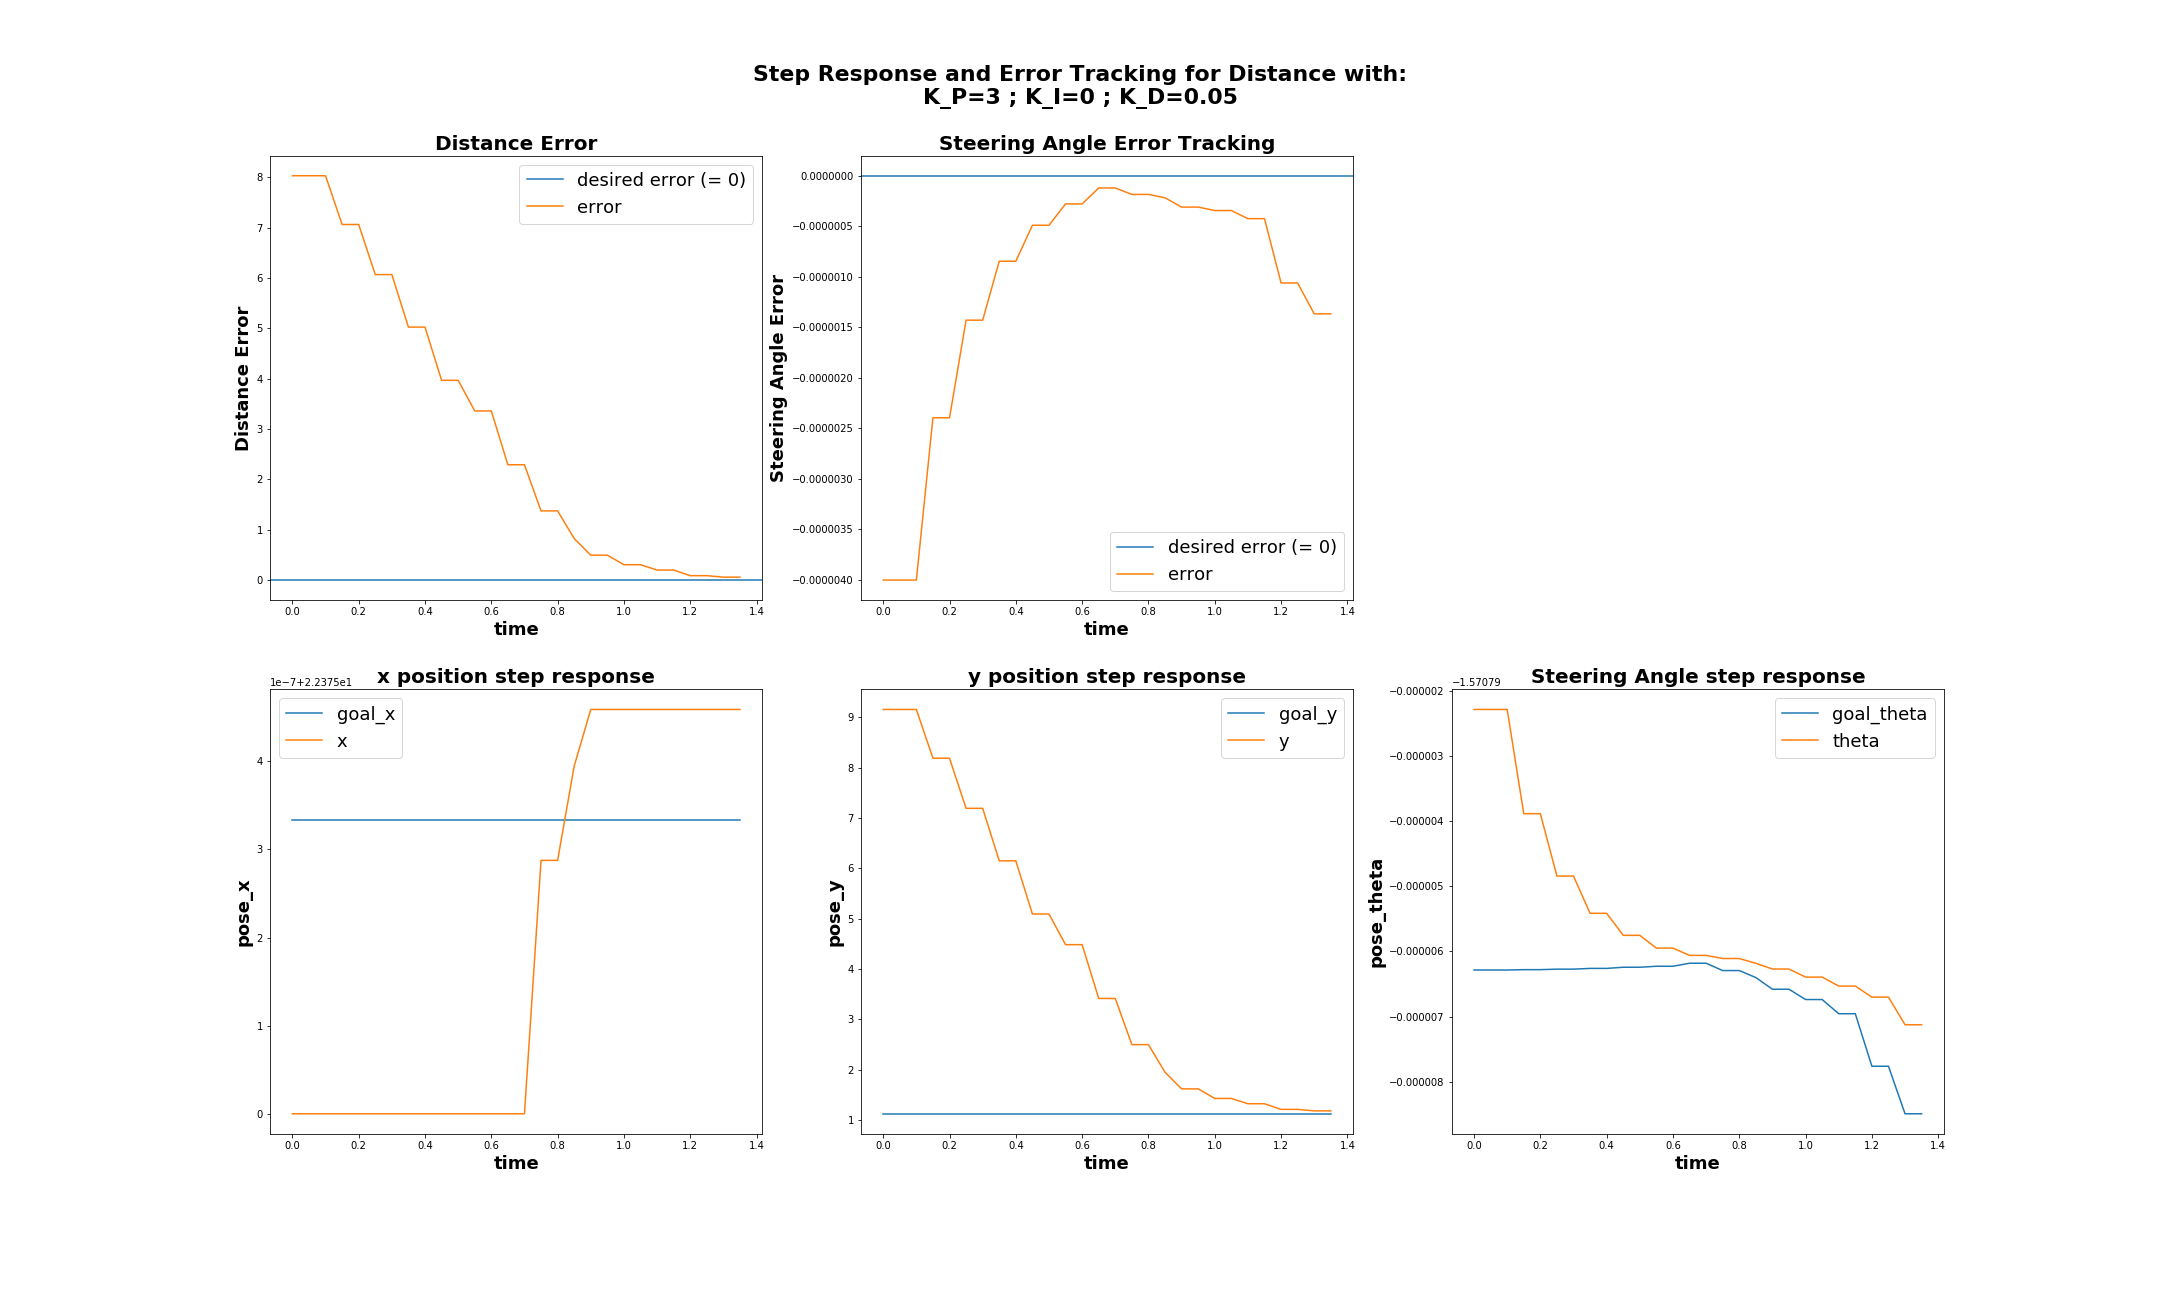
\includegraphics[scale=0.25]{images/control_dist_3_0_0.05.png}\\
	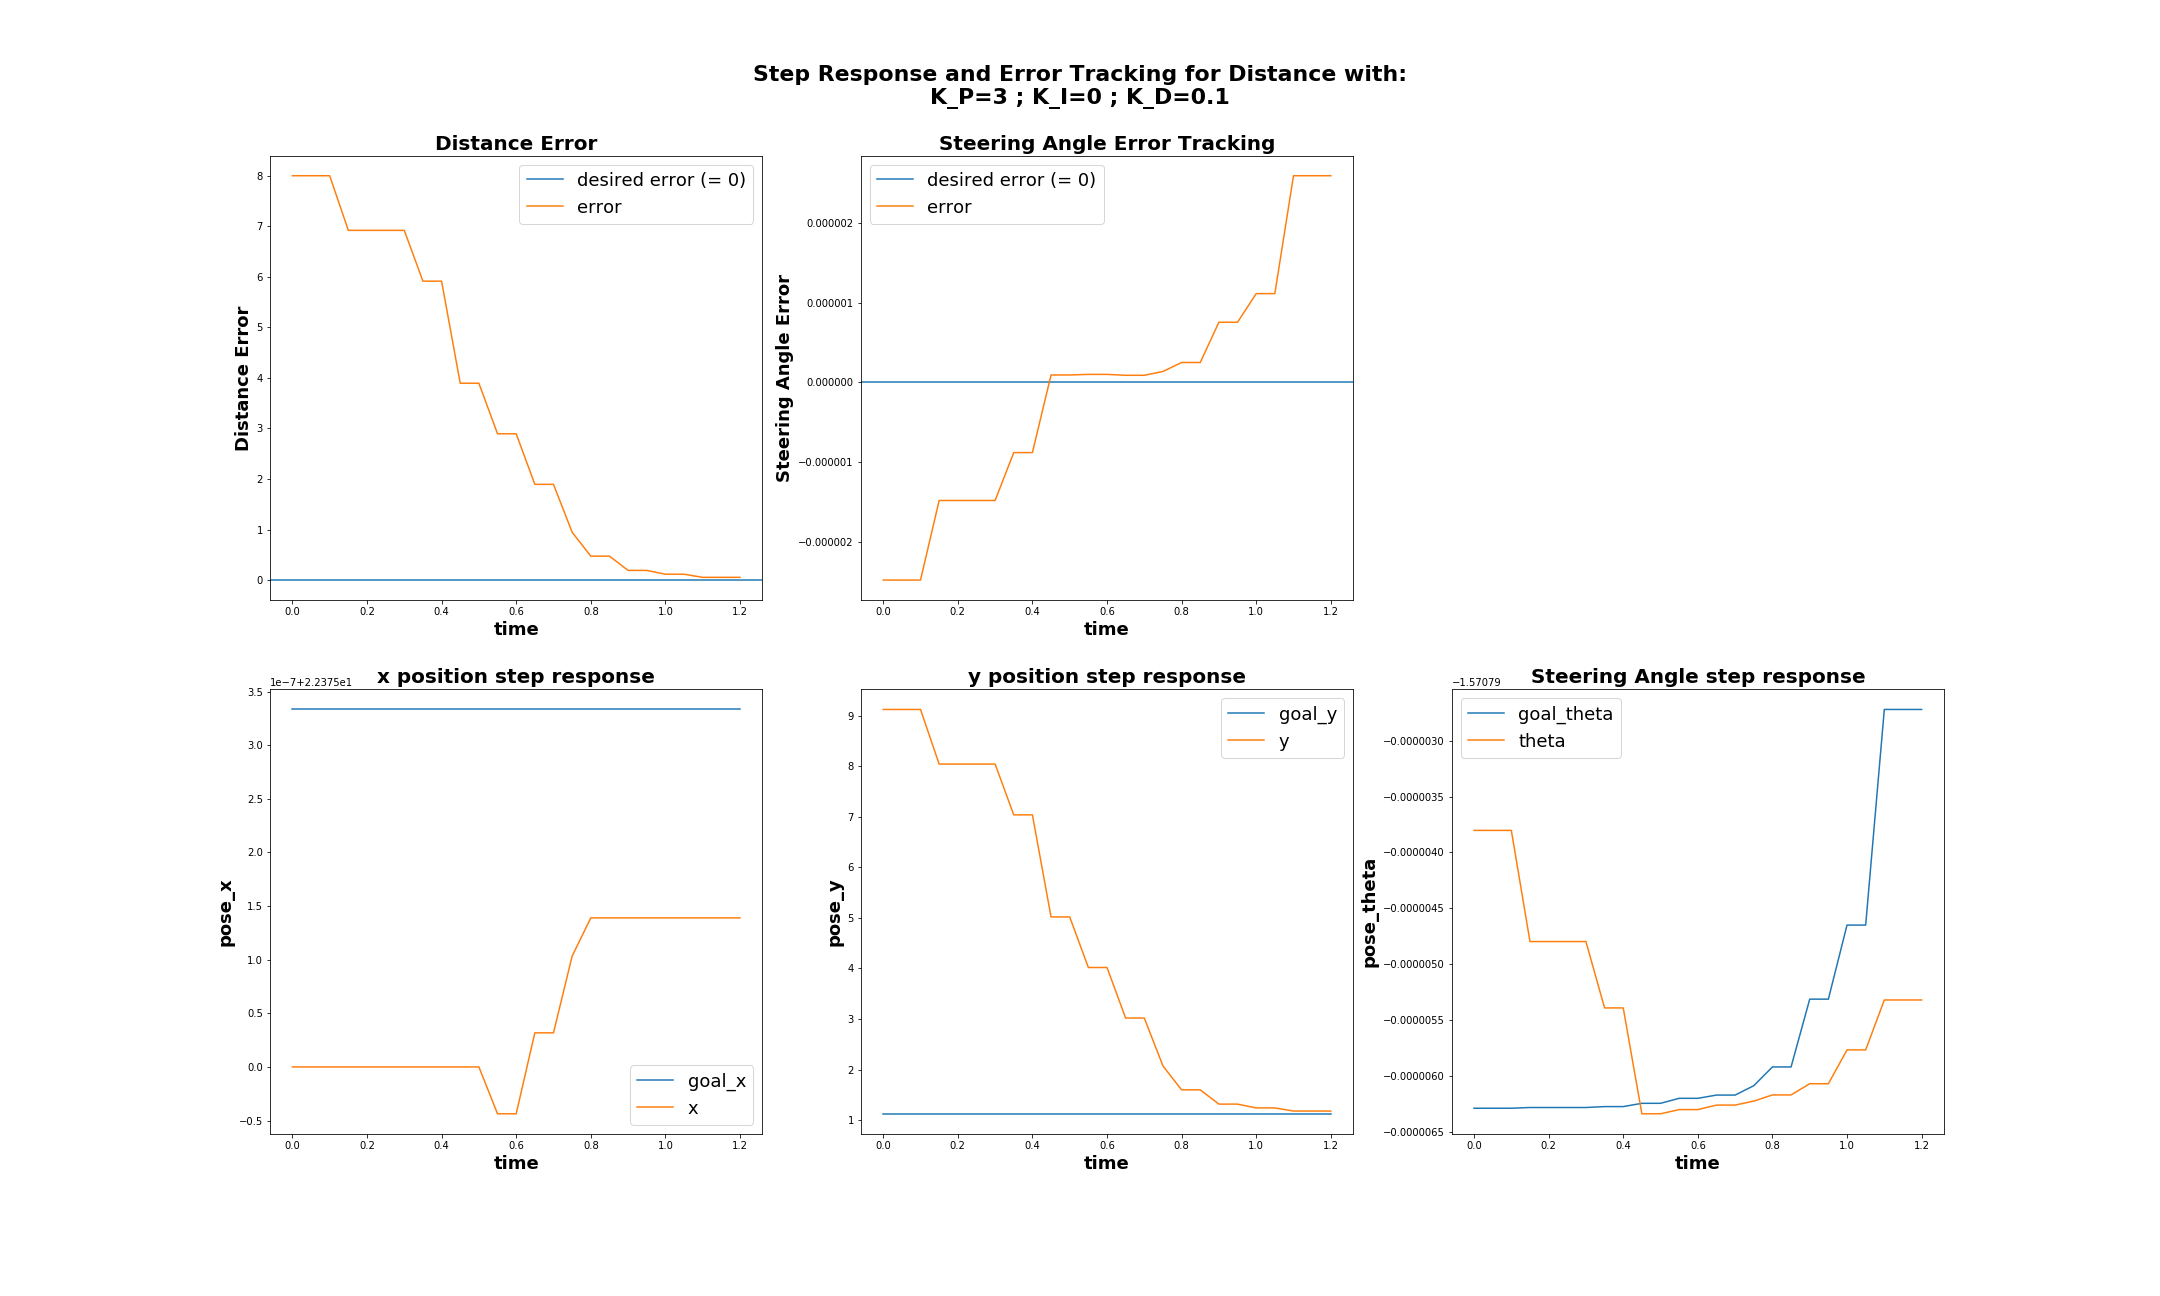
\includegraphics[scale=0.25]{images/control_dist_3_0_0.1.png}
	\subsection{Angular Orientation Controller}
3	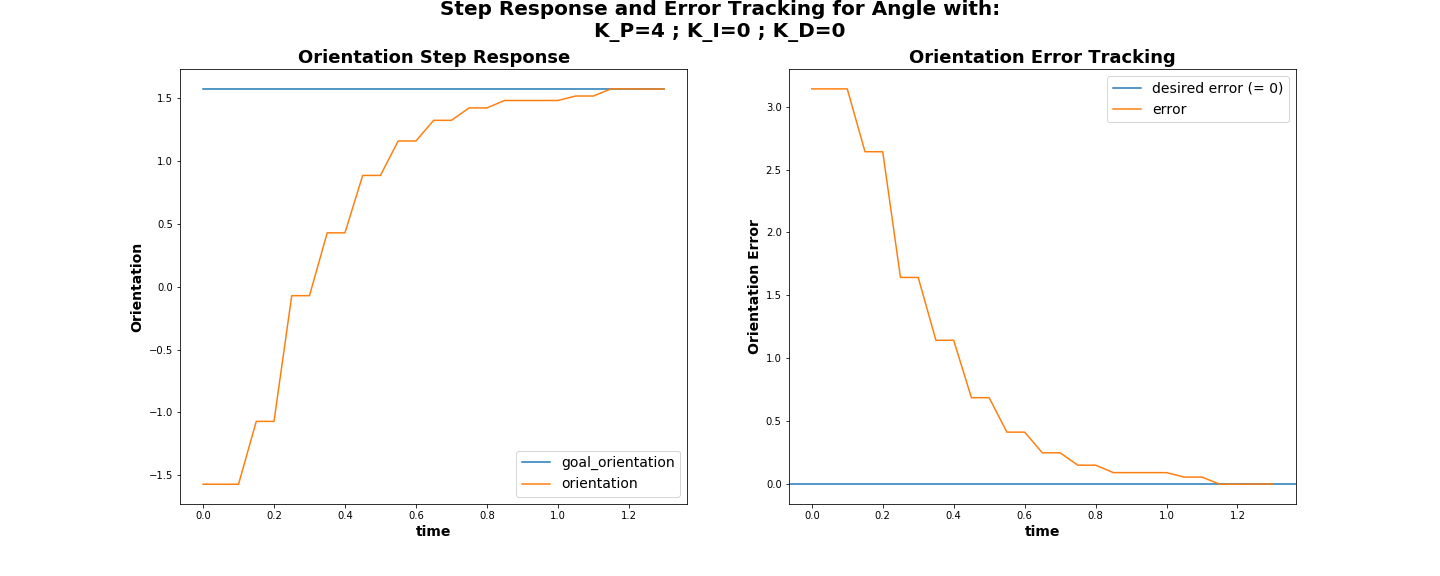
\includegraphics[scale=0.4]{images/control_ang_4_0_0.png}
	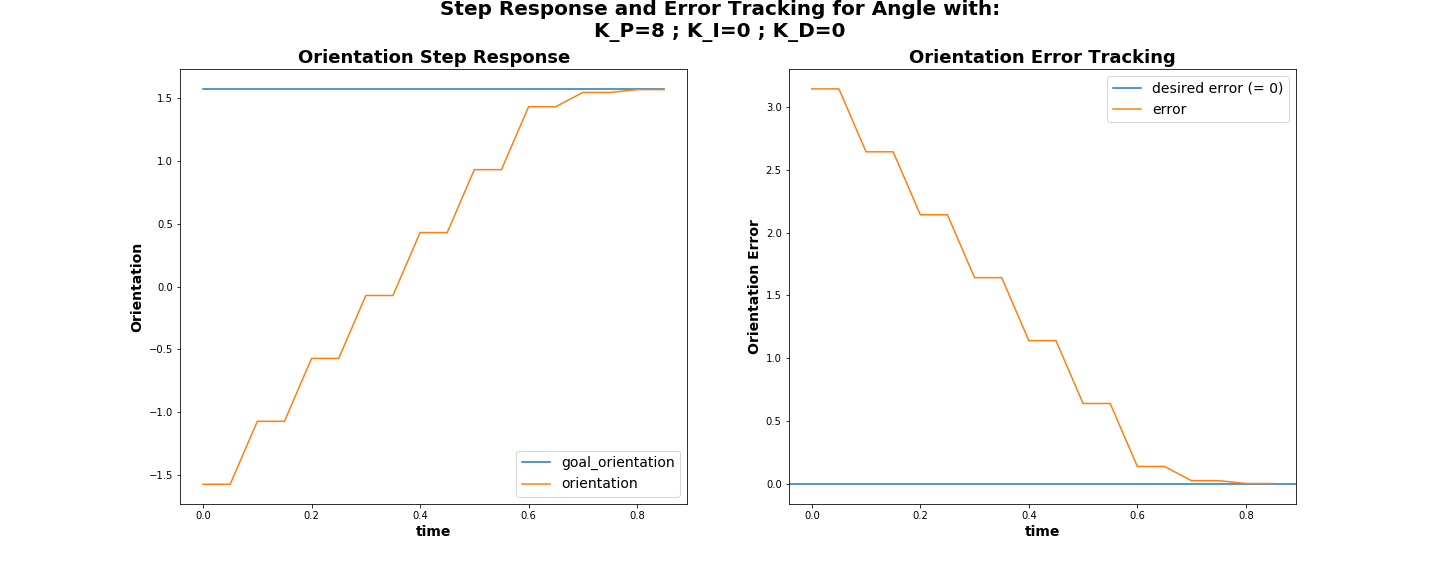
\includegraphics[scale=0.4]{images/control_ang_8_0_0.png}
	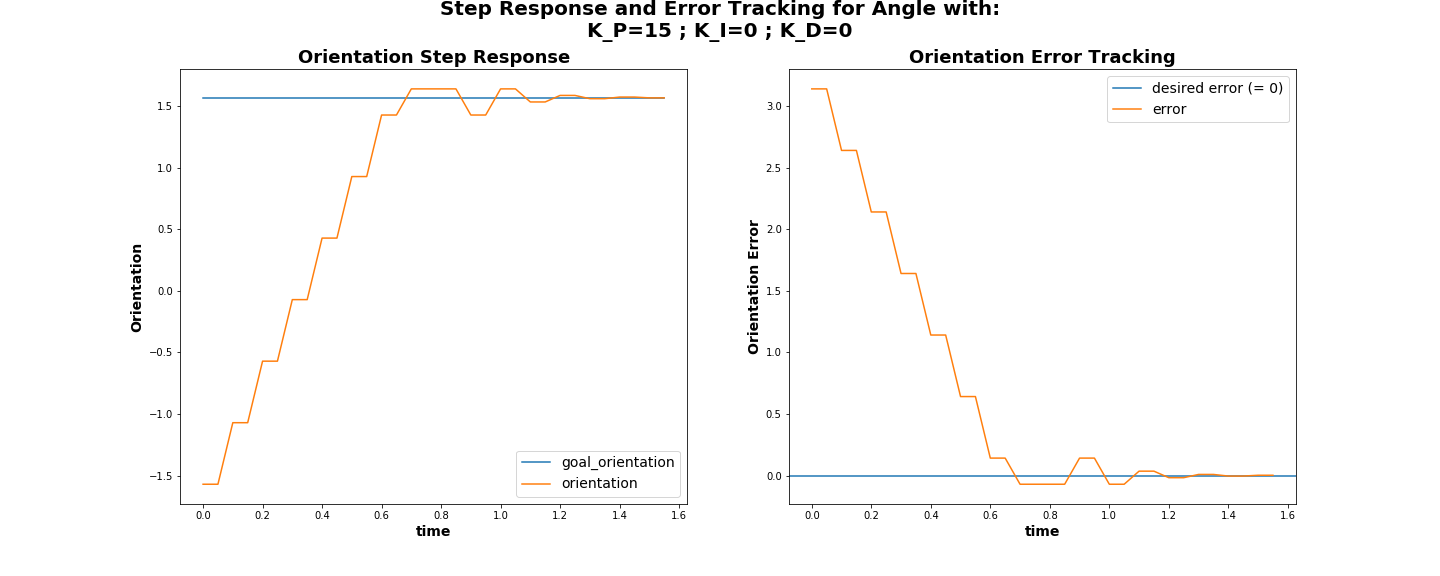
\includegraphics[scale=0.4]{images/control_ang_15_0_0.png}
	\\
	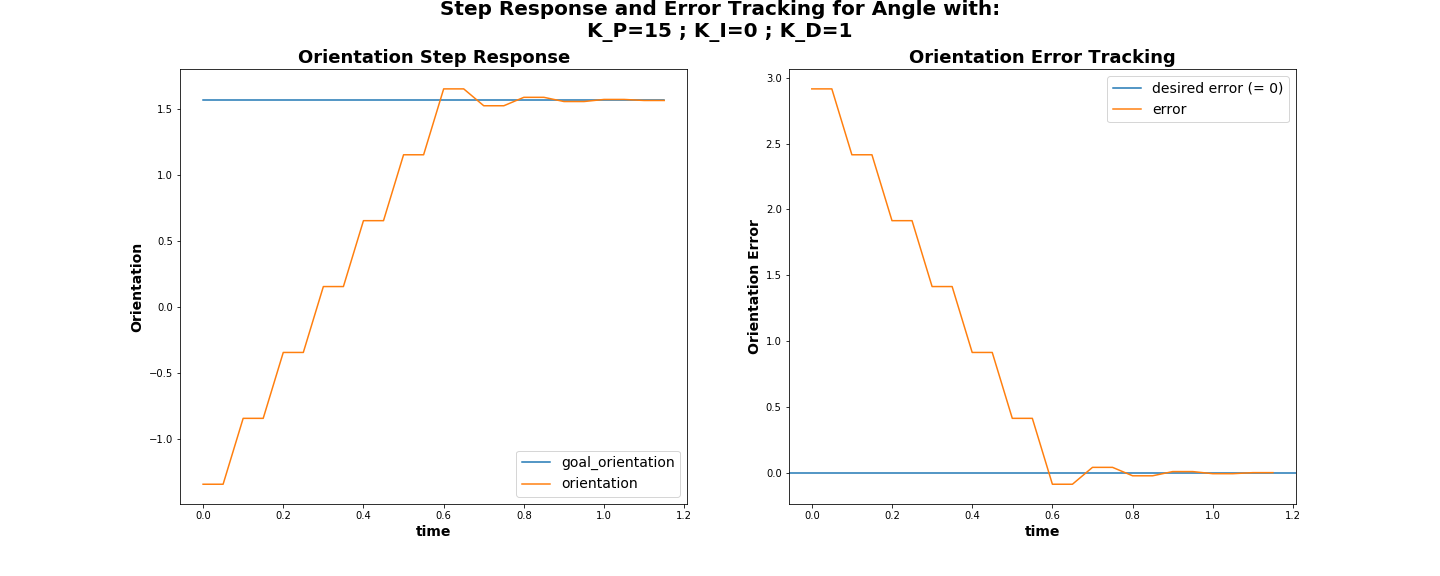
\includegraphics[scale=0.4]{images/control_ang_15_0_1.png}
	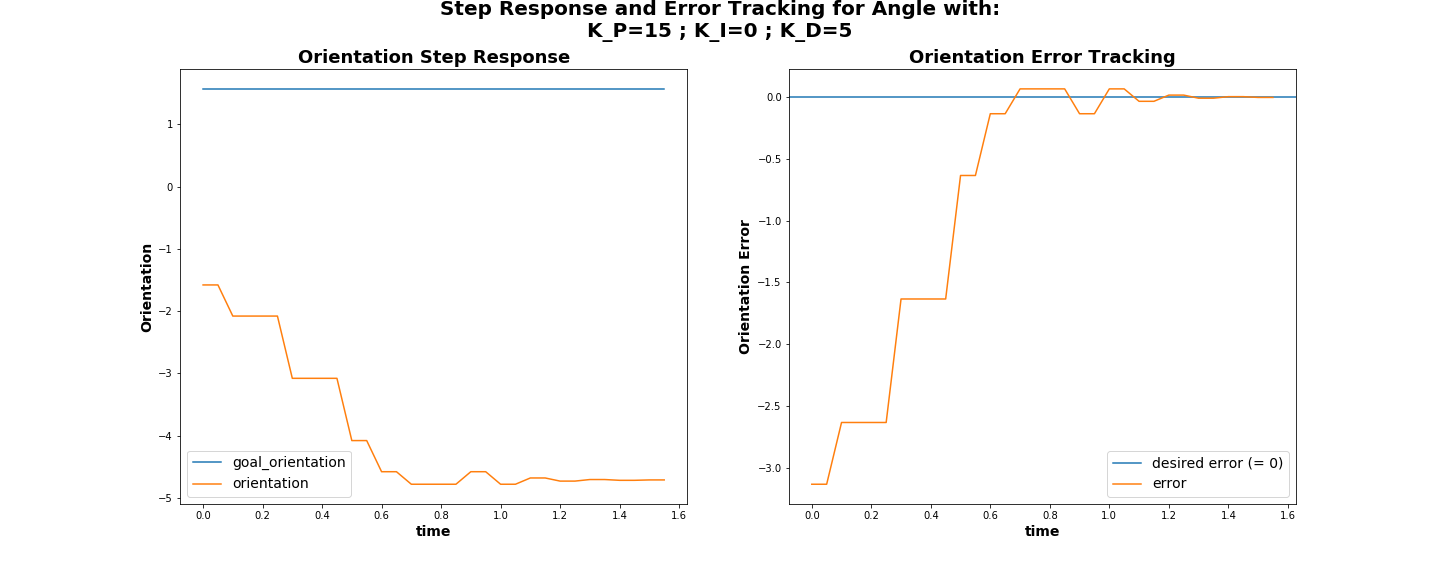
\includegraphics[scale=0.4]{images/control_ang_15_0_5.png}
	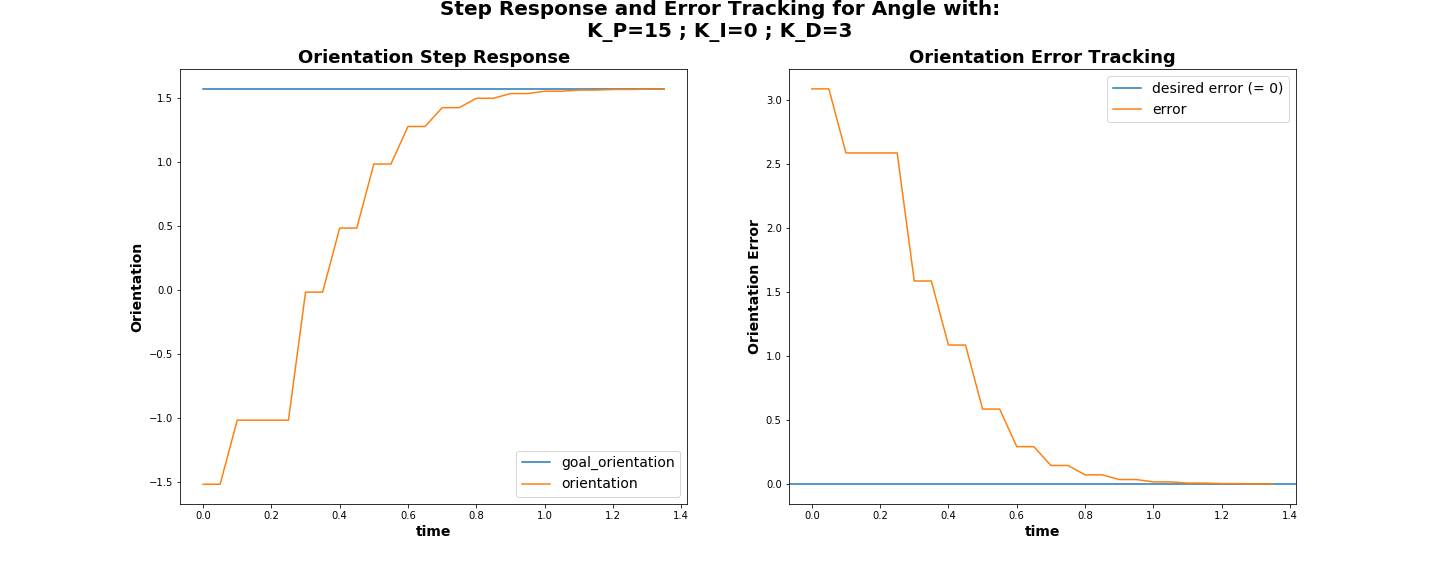
\includegraphics[scale=0.4]{images/control_ang_15_0_3.png}
	
\end{document}